% Copyright (C) 2007 Technical University of Liberec.  All rights reserved.
%
% Please make a following reference to Flow123d on your project site if you use the program for any purpose,
% especially for academic research:
% Flow123d, Research Centre: Advanced Remedial Technologies, Technical University of Liberec, Czech Republic
%
% This program is free software; you can redistribute it and/or modify it under the terms
% of the GNU General Public License version 3 as published by the Free Software Foundation.
%
% This program is distributed in the hope that it will be useful, but WITHOUT ANY WARRANTY;
% without even the implied warranty of MERCHANTABILITY or FITNESS FOR A PARTICULAR PURPOSE.
% See the GNU General Public License for more details.
%
% You should have received a copy of the GNU General Public License along with this program; if not,
% write to the Free Software Foundation, Inc., 59 Temple Place - Suite 330, Boston, MA 021110-1307, USA.
%
%%%%%%%%%%%%%%%%%%%%%%%%%%%%%%%%%%%%%%%%%%%%%%%%%%%%%%%%%%%%%%%%%%
%
% use PDFLatex to compile this
%

\documentclass[a4paper]{article}
\usepackage{amsfonts,amsmath,amsthm,authblk}
\usepackage[bbgreekl]{mathbbol}
\usepackage{stmaryrd}
\usepackage{tikz}
\usepackage{graphicx} %[dvips]
\usepackage[numbers]{natbib}
\usepackage{ mathrsfs }
\usepackage{subcaption}
\usepackage{titlesec} % for \titleformat
\usepackage{mathtools}
\mathtoolsset{centercolon}

\usepackage[colorlinks,citecolor=red,urlcolor=blue,bookmarks=false,hypertexnames=true]{hyperref} 


%%%%%%%%%%%%%%%%%%%%%%%%%%%%%%%%%%%%%%%%%%%%%%%%%%%%%%%%%%%%%%%%%%%%%%%%%%%%
\newtheorem{theorem}{Theorem}[section]
\newtheorem{corollary}[theorem]{Corollary}
\newtheorem{lemma}[theorem]{Lemma}
\newtheorem*{remark}{Remark}
\numberwithin{equation}{section}

%%%%%%%%%%%%%%%%%%%% authors' specific math macros
\def\adiv{\widetilde\div}
\def\aep{\tilde\ep}
\def\agrad{\widetilde\nabla}
\def\avg#1{\left\{\mskip-5mu\left\{#1\right\}\mskip-5mu\right\}}
\def\bbeta{\boldsymbol{\beta}}
\def\CC{\tn C}
\def\d {\,{\rm d}}
\def\ddt#1{\frac{\d #1}{\d t}}
\def\div{\operatorname{div}}
\def\dt{\prtl_t}
\def\dual#1#2{\left\langle #1,#2\right\rangle}
\def\ee{\vc e}
\def\ep{\boldsymbol\varepsilon}
\def\erfc{\operatorname{erfc}}
\def\FF{\vc F}
\def\ff{\vc f}
\def\Hf{\mathscr{L}} % Lebesgue space for flow
\def\jmp#1{\left\llbracket #1 \right\rrbracket}
\def\nn{\vc n}
\def\nnu{\boldsymbol\nu}
\def\norm#1{\left\|#1\right\|}
\def\pbar{\overline p}
\def\pphi{{\varphi}}
\def\prtl{\partial}
\def\qq{\vc q}
\def\Real{{\mathbf R}} % set of all real numbers
\def\tn#1{{\mathbb{#1}}}    % tensor
\def\ttraction{\vc t}
\def\U{\vc U}
\def\ubar{\overline\uu}
\def\uu{\vc u}
\def\V{\vc V}
\def\Vel{{\boldsymbol{\mathcal V}}} % Sobolev space for elasticity
\def\Vf{{\mathcal V}} % Sobolev space for flow
\def\vc#1{\mathbf{#1}}     % vector
\def\vv{\vc v}
\def\weakly{\rightharpoonup}
\def\wh{\widehat}
\def\xx{\vc x}
\def\yy{{\vc y}}

% plus and minus in circle
\newcommand{\opm}{
  {\mathbin{
    \mathchoice
      {\buildcirclepm{\displaystyle     }{0.14ex}{0.95}{0.05ex}{.7}}
      {\buildcirclepm{\textstyle        }{0.14ex}{0.95}{0.05ex}{.7}}
      {\buildcirclepm{\scriptstyle      }{0.13ex}{0.955}{0.04ex}{.55}}
      {\buildcirclepm{\scriptscriptstyle}{0.08ex}{0.95}{0.03ex}{.45}}
  }} 
}
\newcommand\buildcirclepm[5]{%
  \begin{tikzpicture}[baseline=(X.base), inner sep=-#5, outer sep=-.65]
    \node[draw,circle,line width=#4] (X)  {\footnotesize\raisebox{#2}{\scalebox{#3}{$#1\pm$}}};
  \end{tikzpicture}%
}

% abbreviations of equation environments
\newcommand{\eq}[1]{\begin{equation}#1\end{equation}}
\newcommand{\eqs}[1]{\begin{equation*}#1\end{equation*}}
\newcommand{\ml}[1]{\begin{multline}#1\end{multline}}
\newcommand{\mls}[1]{\begin{multline*}#1\end{multline*}}

%%%%%%%%%%%%%%%%%%%% end authors' specific math macros

\def\jb#1{NOTE JB: {\color{violet}#1}}
\def\js#1{NOTE JS: {\color{blue}#1}}

%%%%%%%%%%%%%%%%%%%%%%%%%%%%%%%%%%%%%%%%%%%%%%%%%%%%%%%%%%%%%%%%%%%%%%%%%%%%%%%%%%%%%%%%%%%%% BEGIN DOCUMENT
\begin{document}

\title{Mixed-dimensional model of poroelasticity}
\author{Jan Březina}
\author{Jan Stebel}
\affil{Institute of New Technologies and Applied Informatics\authorcr
Faculty of Mechatronics, Informatics and Interdisciplinary Studies\authorcr
% Technical University of Liberec
% \authorcr
% and\authorcr
% Department of Nanotechnology and Informatics\authorcr
% Institute for Nanomaterials, Advanced Technologies and Innovation\authorcr
Technical University of Liberec\authorcr
Studentská 1402/2, 461 17 Liberec, Czech Republic\authorcr
\texttt{\{jan.brezina,jan.stebel\}@tul.cz}}
% \date{April 3, 2020}
\maketitle

\begin{abstract}
The paper provides derivation and analysis of a poroelasticity model in a domain with fracture represented by a codimension-one manifold. The system of saturated flow and linear elasticity both in the matrix domain and in the fracture coupled through appropriate interface condition is obtained from a continuum description by integration and semi-discretization in the normal direction of the fracture.
The existence and uniqueness of a weak solution are proved with the help of a fixed-point argument.
The analysis is complemented by a numerical example.
\end{abstract}

\paragraph{Keywords:}
Biot's poroelasticity, discrete fracture-matrix model, fixed-stress splitting.

\paragraph{2010 Mathematics Subject Classification:}
35M33, % Initial-boundary value problems for mixed-type systems of PDEs
35Q86, % PDEs in connection with geophysics
74S05, % Flows in porous media; filtration; seepage
74F10. % Fluid-solid interactions (including aero- and hydro-elasticity, porosity, etc.)
% 74B05, % Classical linear elasticity
% 74G25, % Existence of solutions of equilibrium problems in solid mechanics


\section{Introduction}
The hydromechanical (HM) interaction of fluid flow and rock mechanics plays a significant role in many important applications such as geothermal power utilization, nuclear waste deposition, or CO${}_2$ storage \cite{rutqvist2003role}. The linear poroelastic model introduced by Biot \cite{biot1941general}, as well as some of its more recent non-linear extensions \cite{rutqvist2003role,Jing2007Fluid} are formulated for a continuum description of fractured rock. The fracture network consists of fractures ranging from grain size cracks of a sub-milimeter scale to fault zones of a kilometer-scale \cite{Bonnet2001}. The small-scale fractures can be described in terms of an equivalent continuum \cite{Oda1986,Rutqvist2013a}. However, the very high aspect ratio (size over aperture) of the fractures leads to large gradients of the principal unknowns, typically flow velocity and displacement, that can not be resolved by classical discretization methods (FVM, FEM). On the other hand, the \textit{discrete fracture network} (DFN) approach \cite{Follin2014methodology,Hyman2015dfnWorks} that describes individual fractures as codimension-one manifolds is unable to treat a vast number of small-scale fractures. Various hybrid approaches are used to combine continuum and discrete fractures; we refer to \cite{Jing2002} for an overview and to \cite{Zhao2013Impact} for numerical comparison of selected approaches. 

As the fracture apertures are still far from the scale of individual molecules, the continuum models of the HM processes derived from fundamental conservation laws are physically reasonable. The limiting factor is the representation of the heterogeneities due to fractures  at the discrete level.

The \textit{discrete fracture-matrix} (DFM) models, also called \textit{mixed-dimensional}, are derived from the continuum model by a \emph{semi-discretization} of the governing equations on the fracture domain
in the normal direction. The fracture domain of the resulting equations is reduced to a codimension-one manifolds, similarly to the DFN approach. The reduction of the fracture domain's dimension leads some authors to name the process \emph{dimension reduction}. However, that term has a quite different meaning in the data processing. In order to avoid confusion, we rather use the term semi-discretization further on.

This technique was used by Martin et al. \cite{martin_modeling_2005} for Darcy flow equations in domains with a single fracture.
Later, the model was extended by \cite{angot2009asymptotic} for immersed, polygonal fracture with variable aperture. The models with intersections and junctions and extension to the transport problems were analyzed in \cite{maryska2005numerical,pichot2012generalized,formaggia2014reduced, schwenck2015dimensionally}. 
Mixed-dimensional poroelasticity models were studied e.g., in \cite{ganis2014modeling} where Biot's system in the matrix was coupled with fracture flow based on the cubic law.
In \cite{hanowski2018hydromechanical} the Biot system in the matrix is coupled with Darcian fracture flow; in addition, fracture width and length can vary according to rock deformation.
There are not so many papers dealing with the mechanics in the fracture.
A general framework for mixed-dimensional elliptic equations was developed in \cite{boon2019stable, boon2017functional} and applied to linear elasticity systems.
We also mention the work \cite{mikelic2019derivation} where a shell model is derived for a poroelastic membrane.

The purpose of the present paper is threefold:
First, we derive the DFM model of poroelasticity in a domain separated by a fracture, using the semi-discretization process for the Biot system.
To cope with the fact that the mechanical part \eqref{eq:lin_el} of the problem is a vector-valued problem, we develop a particular calculus for tangential and normal parts of functions and operators.
In contrast to other works, we consider general conductivity and elasticity tensors not necessarily aligned with the fracture orientation.
The obtained equations are expressed in terms of mean pressure and mean displacement in the fracture.
The resulting problem consists of equations of flow and mechanics in the fracture and the surrounding domain, accompanied by appropriate interface conditions.

The second aim of the paper is to analyze the well-posedness of the mixed-dimensional poroelasticity.
There are two main strategies for solving poromechanics systems: monolithic methods (see e.g. \cite{showalter2000diffusion,zenisek1984existence}) and iterative splittings.
The latter approach has a significant advantage in the design of numerical schemes where the splitting acts as a preconditioner \cite{white2016block} that allows sequential use of different solvers for flow and mechanics.
Here we follow the optimized fixed-stress iterative splitting analyzed in \cite{mikelic2013convergence}, and show the contractivity of the appropriate mapping.% with optimal estimates of splitting parameters.

The third aim is to apply the mixed-dimensional model in the numerical solution of a simple test problem.
We perform a simulation of the problem of fluid injection into the fracture, verify the results against an analytical solution and test the robustness of the fixed-stress splitting method.

The structure of the paper is as follows.
In section \ref{sec:model}, we describe the full and reduced geometry and the unreduced Biot poroelasticity model.
Then in section \ref{sec:calculus}, we present the tangential and normal calculus, which will be used in the semi-discretization process in section \ref{sec:dim_red}.
The process results in the reduced DFM model \eqref{eq:mixed_dim_problem} describing  flow and mechanics in matrix and fracture with appropriate interface conditions.
% We further formulate a modified problem \eqref{eq:mixed_dim_perm}, which is valid under the assumption of permeable fracture.
In section \ref{sec:well_pos}, we analyze the existence and uniqueness of the solution to this problem, first studying the mechanics and flow equations separately and combining them later in the iterative scheme.
Finally, in section \ref{sec:comp_test}, we describe the computational test problem, its discretization and present the computational results.



\section{Biot's poroelasticity in domain with fracture}\label{sec:model}
Let $\Omega$ be a bounded, simply connected domain in the Euclidean space $\Real^d$, $d\in\{2,3\}$, with Lipschitz boundary $\partial\Omega$.
We assume that $\Omega$ is composed of two subdomains: the matrix $\Omega_m$ and the fracture $\Omega_f:=\Omega\setminus\overline\Omega_m$ that separates the matrix into two parts (see Figure \ref{fig:omegas}). 
\begin{figure}[h]
\centering
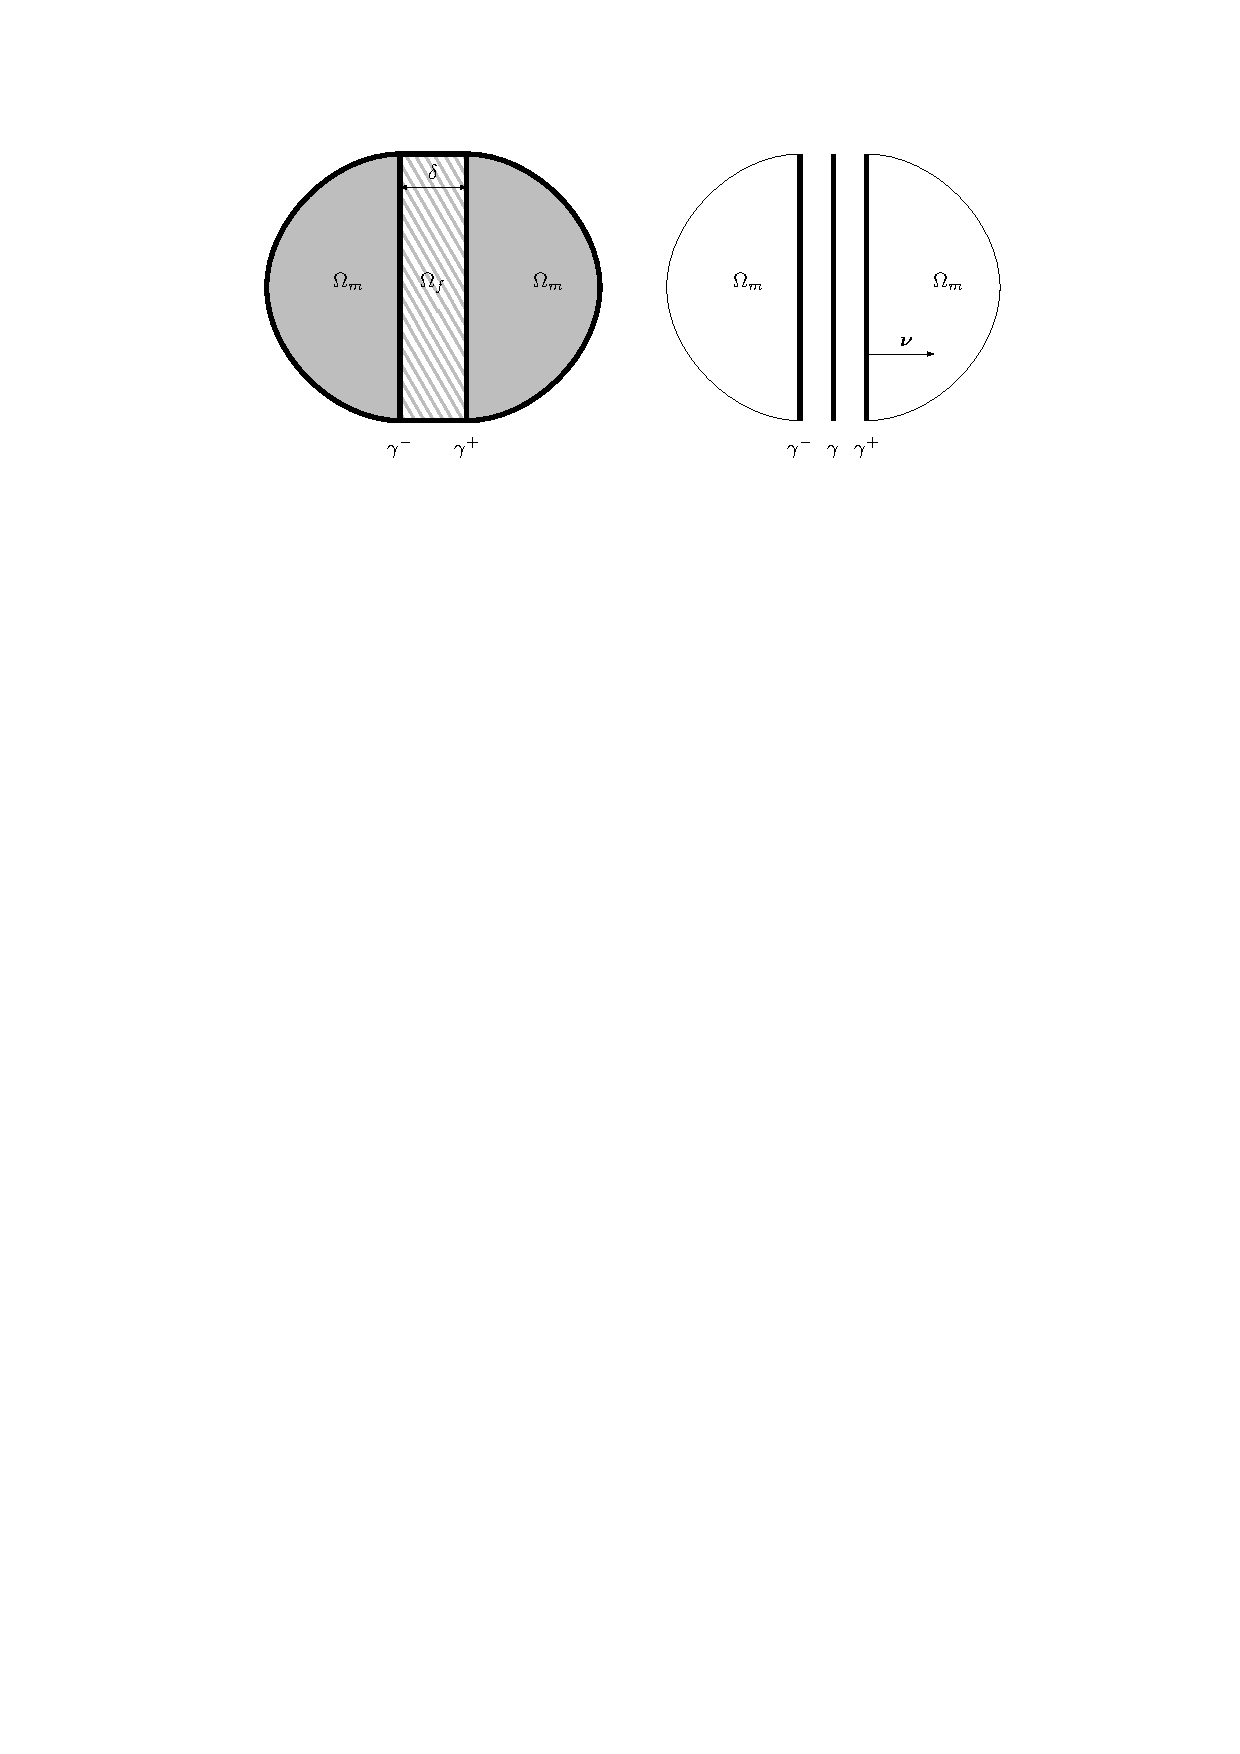
\includegraphics[width=\textwidth]{figures/omegas}
\caption{The domain of the full model (left) and the reduced geometry (right).}
\label{fig:omegas}
\end{figure}

We assume that the fracture domain have form of a neighbourhood of a manifold; we consider hyperplane in $\Real^d$ for the sake of simplicity. On the hyperplane with normal $\nnu$,  we consider a domain $\gamma$ and the fracture aperture $\delta > 0$, possibly dependent on $\vc x$. Then the fracture domain is assumed in the form:
\eqs{ \Omega_f = \{\xx+s\nnu;~\xx\in\gamma,~s\in(-\tfrac\delta2,\tfrac\delta2)\}. } 

The two parts of $\Omega_m$ are interacting with $\Omega_f$ via the interfaces
\eqs{ \gamma^+ := \{\xx+\tfrac\delta2\nnu;~\xx\in\gamma\},\quad \gamma^- := \{\xx-\tfrac\delta2\nnu;~\xx\in\gamma\}. }
The symbol $\prtl\gamma$ shall denote the relative boundary of the domain $\gamma$ with respect to the hyperplane. In the rest of this section, we shall describe the Biot system \cite{biot1941general} on the domain $\Omega$ in the equivalent form of the separate equations in $\Omega_m$ and $\Omega_f$ coupled through the continuity conditions on the interfaces $\gamma^\pm$. The reduced system of equation on $\Omega_m$ and $\gamma$ is derived later in section $\ref{sec:dim_red}$.

Let $I=(0,T)$ be a finite time interval, the balance of mass and forces in matrix and fracture is given by the equations
\begin{subequations}
\label{eq:biot}
\begin{align}
    \label{eq:lin_el}
    -\div \bbsigma + \nabla(\alpha p) &= \ff &&\mbox{ in }I\times(\Omega_m\cup\Omega_f),\\
\label{eq:biot_darcy}    \dt\left(Sp + \div(\alpha\uu)\right) + \div\qq &= g &&\mbox{ in }I\times(\Omega_m\cup\Omega_f).
\end{align}
Here, the displacement $\uu$ and the pressure $p$ are the principal unknowns; further $\alpha$ is the Biot effective stress parameter, $S$ the storativity,
 $\ff$ the density of body force, and $g$ the density of fluid source.
The stress tensor $\bbsigma$ and the flux $\qq$ are determined by the Hooke and Darcy law, respectively:
\eqs{ \bbsigma = \CC\nabla\uu, \quad \qq = -\tn K\nabla p, }
via the $4^{\rm th}$-order elasticity tensor $\CC$ and the hydraulic conductivity tensor $\tn K$.
We consider the initial condition for the given initial pressure $p_0$ and simple homogeneous Dirichlet boundary conditions:
\begin{align}
p(0,\cdot) &= p_0 &&\mbox{ in }\Omega_m\cup\Omega_f,\\
p &= 0,\quad \uu=\vc 0 &&\mbox{ on }I\times\prtl\Omega.
\end{align}
To complete the system of equations, we have to specify interface conditions between matrix and fracture.
To this end, we choose conditions equivalent to the piecewise heterogenous medium:
\eq{ \label{eq:continuity_on_gamma_pm} p,\uu,\qq\cdot\nnu,\bbsigma\nnu-\alpha p\nnu \mbox{ are continuous on } I\times\gamma^\pm. }
% For detailed discussion and other possible conditions, we refer to \cite{deresiewicz-skalak,gurevich-schoenberg}.
\end{subequations}

In what follows, we shall assume that the physical parameters $\alpha,S,\CC,\tn K$ are constant in $\Omega_m$, $\Omega_f$, respectively.
To distinguish values in $\Omega_m$ and $\Omega_f$, we shall use the subscripts ``$m$'' and ``$f$'', i.e. $\alpha_m := \alpha_{|\Omega_m}$, $\alpha_f := \alpha_{|\Omega_f}$ etc.
We also impose standard requirements for the data:
\begin{itemize}
\item $\alpha_*\ge 0$, $S_*>0$ for $*\in\{m,f\}$;
\item $\CC_*$ and $\tn K_*$, $*\in\{m,f\}$, have the usual symmetries:
\eqs{ \forall \tn A,\tn B\in\Real^{d\times d}:~ \CC_*\tn A:\tn B=\CC_*\tn A^\top:\tn B=\CC_*\tn A:\tn B^\top=\CC_*\tn B:\tn A, }
\eqs{ \tn K_* = \tn K_*^\top; }
\item $\CC_*$ and $\tn K_*$, $*\in\{m,f\}$, are positive definite: % \cite{gurtin}:
There exist positive constants $\mu_m$, $\mu_f$, $\lambda_m$, $\lambda_f$, $\kappa_m$, $\kappa_f$, such that
\eq{ \label{eq:pos_def_C_gen} \forall\tn A\in\Real^{d\times d}:~\CC_*\tn A:\tn A \ge \mu_*\left|\tn A+\tn A^\top\right|^2 + \lambda_*|\tn I:\tn A|^2, }
\eq{ \label{eq:pos_def_K} \forall\vv\in\Real^d:~\tn K_*\vv\cdot\vv \ge \kappa_*|\vv|^2,\quad *\in\{m,f\}. }
\end{itemize}
Here ``:'' stands for the scalar product in $\Real^{d\times d}$ and $|\tn A|$ denotes the Frobenius norm, i.e. $|\tn A|^2=\tn A:\tn A$.

In addition to the above assumptions on the data, we shall restrict ourselves to the case of highly permeable fracture, i.e.
\eq{\label{eq:asm_permeable_frac} |\tn K_m|\ll \kappa_f. }
In such situations it is typical that pressure variations across the fracture are very small.


\section{Preliminaries}\label{sec:calculus}

In this section we introduce notation and tools that will be used later in the derivation of the mixed-dimensional Biot system.

\subsection{Tangential and normal calculus}
Let $\tn P := \nnu\otimes\nnu = [\nu_i\nu_j]_{i,j=1}^d$ be the orthogonal projector to $\gamma$.
For any vector $\vv\in\Real^d$ we introduce the orthogonal decomposition into normal and tangential direction to $\gamma$:
\eqs{ \vv = \vv_\nu + \vv_\tau, \mbox{ where } \vv_\nu := \tn P\vv \mbox{ and } \vv_\tau := (\tn I-\tn P)\vv. }
% In the rest of this section, $f$, $\vv$, $\tn A$ will be scalar-, vector- and tensor-valued functions defined in $\overline\Omega_f$.
% Let $f$ be a scalar function defined in $\overline\Omega_f$.
% The gradient and divergence operators in $\gamma$ are decomposed into the normal and tangential part as follows:
The gradient operator of a function $f$, is decomposed into the normal and tangential part as follows:
\eqs{ \nabla f = (\nabla f)_\nu + (\nabla f)_\tau =: \nabla_\nu f + \nabla_\tau f. }
We note that since the tangential gradient does not depend on values outside of $\gamma$, it is well-defined even for functions defined only in $\gamma$.

For vector- and tensor-valued functions we use analogous notation.
In particular, tensors are decomposed to normal and tangential parts as follows:
\eqs{ \tn A = \tn A\tn P + \tn A(\tn I-\tn P) =: \tn A_\nu + \tn A_\tau. }
Accordingly, we split the gradient of a vector-valued function:
\eqs{ \nabla\vv = (\nabla\vv)_\nu + (\nabla\vv)_\tau =: \nabla_\nu\vv + \nabla_\tau\vv. }
The divergence operators are decomposed as follows:
\begin{align*}
% \tn A &= \tn A\tn P + \tn A(\tn I-\tn P) =: \tn A_\nu + \tn A_\tau,\\
% \nabla\vv &= (\nabla\vv)_\nu + (\nabla\vv)_\tau =: \nabla_\nu\vv + \nabla_\tau\vv,\\
\div\vv &= \div\vv_\nu + \div\vv_\tau =: \div_\nu\vv + \div_\tau\vv,\\
\div\tn A &= \div(\tn P\tn A) + \div((\tn I-\tn P)\tn A) =: \div_\nu\tn A + \div_\tau\tn A.
\end{align*}
We recall that the components of the Jacobian matrix and of the tensor divergence are given by $\nabla\vv=\left[\tfrac{\prtl v_i}{\prtl x_j}\right]_{i,j=1}^d$ and $\div\tn A = \left[\sum_{j=1}^d\tfrac{\prtl a_{ij}}{\prtl x_j}\right]_{i=1}^d$, respectively.

Green's identity in $\gamma$ reads:
\eqs{ \int_\gamma(\div_\tau\vv)f = \int_{\prtl\gamma}(\vv\cdot\nn)f - \int_\gamma\vv\cdot\nabla_\tau f, }
where $\nn$ denotes the unit outward normal to $\partial\gamma$.


\subsection{Averages, jumps and approximate gradients}
The symbols $f^\oplus$ and $f^\ominus$ will denote the trace of $f$ on $\gamma^+$, $\gamma^-$, respectively, i.e.
\eqs{ f^{\opm}(\xx) := f(\xx\pm\tfrac\delta2\nnu), ~\xx\in\gamma. }
Using these symbols, we can introduce the average and jump operators:
\eqs{ \avg{f} := \frac{f^\oplus+f^\ominus}2,\quad \jmp{f} := f^\oplus-f^\ominus. }
% The same notation will be used for vector- and tensor-valued functions.
By $\overline f$ we shall denote the integral mean of $f$ across the fracture aperture, i.e.
\eqs{ \overline f(\xx):=\frac1\delta\int_{-\tfrac\delta2}^{\tfrac\delta2} f(\xx+s\nnu) \d s,~\xx\in\gamma. }
For a pair of functions $f:\gamma^+\cup\gamma^-\to\Real$ and $F:\gamma\to\Real$ we define the approximate gradient operator in the positive and negative half of fracture as follows:
\eqs{ \agrad^\opm(f,F) := \nabla_\tau F \pm \frac2\delta(f^\opm - F)\nnu. }
% \begin{remark}
% In the previous definitions we have used two-point differences to approximate derivatives in the normal direction.
% We note that it is possible to use more general relations using all three values $f^\oplus$, $\overline f$, $f^\ominus$ (see e.g. \cite{martin_modeling_2005}).
% The two-point formulas are suitable for possible generalization at fracture intersections and junctions.
% \end{remark}
% Analogous properties hold for vector- and tensor-valued functions.
% Despite the indicated approximations, the following relations between the integral means and averaged approximates still hold exactly for all admissible functions:
% \eq{\label{eq:agrad_sc} \overline{\nabla f} = \nabla_\tau\overline f + \frac1\delta\jmp{f}\nnu = \avg{\agrad(f,\overline f)}, }
% 
We also introduce the approximate gradient and divergence for vector-valued functions $\vv,\V$:
\eqs{
\agrad^\opm(\vv,\V) := \nabla_\tau\V \pm \frac2\delta(\vv^\opm - \V)\otimes\nnu,\quad
\adiv^\opm(\vv,\V) := \div_\tau\V \pm \frac2\delta(\vv^\opm - \V)\cdot\nnu.
% \adiv^\opm[\tn A,\overline{\tn A}] &:= \div_\tau\overline{\tn A} \pm \frac2\delta(\tn A^\opm - \overline{\tn A})^\top\nnu.
}

\subsection{Identities for averages and gradients}
% The following identities, which will be used in the dimension reduction process, hold true:
The integral means of differential operators satisfy the following relations:
\begin{align}
\label{eq:agrad_sc} \overline{\nabla f} &= \nabla_\tau\overline f + \frac1\delta\jmp{f}\nnu = \avg{\agrad(f,\overline f)}, \\
\label{eq:agrad_vc} \overline{\nabla\vv} &= \nabla_\tau\overline\vv+\frac1\delta\jmp{\vv}\otimes\nnu = \avg{\agrad(\vv,\overline\vv)}, \\
\label{eq:adiv_vc} \overline{\div\vv} &= \div_\tau\overline\vv+\frac1\delta\jmp{\vv}\cdot\nnu = \avg{\adiv(\vv,\overline\vv)}, \\
\label{eq:adiv_tn} \quad \overline{\div\tn A} &= \div_\tau\overline{\tn A} + \frac1\delta\jmp{\tn A^\top}\nnu. % = \avg{\adiv[\tn A,\overline{\tn A}]}. }
\end{align}
For the proof we refer to Appendix \ref{sec:ap_ineq}.
% The above identities relate integral means of differential operators with tangential operators and jumps in the fracture.

Furthermore, for twice continuously differentiable functions $f\in\mathcal C^2(\overline\Omega_f)$, Taylor's expansion implies that
\eq{ \label{eq:approx_Odelta} f^\opm = \overline f + O(\delta), \quad (\nabla f)^\opm = \agrad^\opm(f,\overline f) + O(\delta). }%, \quad \div f^\opm = \adiv[f,\overline f] + O(\delta). }
Here the remainder $O(\delta)$ represents an expression that can be estimated from above by $\delta C\norm{f}_{\mathcal C^2(\overline\Omega_f)}$ where $C>0$ is independent of $f$ and $\delta$.




% \section{Tangential and normal calculus in fracture}\label{sec:calculus}
% 
% In this section we develop tools that will be used later in the derivation of the mixed-dimensional Biot system.
% Let $\tn P := \nnu\otimes\nnu = [\nu_i\nu_j]_{i,j=1}^d$ be the orthogonal projector to $\gamma$.
% For any vector $\vv\in\Real^d$ we introduce the orthogonal decomposition into normal and tangential direction to $\gamma$:
% \eqs{ \vv = \vv_\nu + \vv_\tau, \mbox{ where } \vv_\nu := \tn P\vv \mbox{ and } \vv_\tau := (\tn I-\tn P)\vv. }
% % In the rest of this section, $f$, $\vv$, $\tn A$ will be scalar-, vector- and tensor-valued functions defined in $\overline\Omega_f$.
% % Let $f$ be a scalar function defined in $\overline\Omega_f$.
% % The gradient and divergence operators in $\gamma$ are decomposed into the normal and tangential part as follows:
% The gradient operator of a function $f:\overline\Omega_f\to\Real$, is decomposed into the normal and tangential part as follows:
% \eqs{ \nabla f = (\nabla f)_\nu + (\nabla f)_\tau =: \nabla_\nu f + \nabla_\tau f. }
% Since the tangential gradient does not depend on values outside of $\gamma$, it is well-defined even for functions defined only in $\gamma$.
% The symbols $f^\oplus$ and $f^\ominus$ will denote the trace of $f$ on $\gamma^+$, $\gamma^-$, respectively, i.e.
% \eqs{ f^{\opm}(\xx) := f(\xx\pm\tfrac\delta2\nnu), ~\xx\in\gamma. }
% Using these symbols we can introduce the average and jump operators:
% \eqs{ \avg{f} := \frac{f^\oplus+f^\ominus}2,\quad \jmp{f} := f^\oplus-f^\ominus. }
% % The same notation will be used for vector- and tensor-valued functions.
% By $\overline f$ we shall denote the integral mean of $f$ across the fracture aperture, i.e.
% \eqs{ \overline f(\xx):=\frac1\delta\int_{-\tfrac\delta2}^{\tfrac\delta2} f(\xx+s\nnu) \d s,~\xx\in\gamma. }
% If $f:\gamma^+\cup\gamma^-\to\Real$ and $F:\gamma\to\Real$ then we denote $\wh{f}:=(f,F)$.
% The approximate gradient operator in the positive and negative half of fracture is defined as follows:
% \eqs{ \agrad^\opm\wh f := \nabla_\tau F \pm \frac2\delta(f^\opm - F)\nnu. }
% % \begin{remark}
% % In the previous definitions we have used two-point differences to approximate derivatives in the normal direction.
% % We note that it is possible to use more general relations using all three values $f^\oplus$, $\overline f$, $f^\ominus$ (see e.g. \cite{martin_modeling_2005}).
% % The two-point formulas are suitable for possible generalization at fracture intersections and junctions.
% % \end{remark}
% If $f\in\mathcal C^2(\overline\Omega_f)$, i.e. $f$ is twice continuously differentiable in $\overline\Omega_f$ then from Taylor's expansion we infer that
% \eq{ \label{eq:approx_Odelta} f^\opm = \overline f + O(\delta), \quad (\nabla f)^\opm = \agrad^\opm(f,\overline f) + O(\delta). }%, \quad \div f^\opm = \adiv[f,\overline f] + O(\delta). }
% Here the remainder $O(\delta)$ represents an expression that can be estimated from above by $\delta C\norm{f}_{\mathcal C^2(\overline\Omega_f)}$ and $C>0$ is a constant independent of $f$ and $\delta$.
% % Analogous properties hold for vector- and tensor-valued functions.
% % Despite the indicated approximations, the following relations between the integral means and averaged approximates still hold exactly for all admissible functions:
% % \eq{\label{eq:agrad_sc} \overline{\nabla f} = \nabla_\tau\overline f + \frac1\delta\jmp{f}\nnu = \avg{\agrad(f,\overline f)}, }
% For the proof we refer to Appendix \ref{sec:ap_ineq}.
% % 
% For vector- and tensor-valued functions $\vv:\overline\Omega_f\to\Real^d$, $\tn A:\overline\Omega_f\to\Real^{d\times d}$ we use analogous notation.
% In particular, tensors are decomposed to normal and tangential parts as follows:
% \eqs{ \tn A = \tn A\tn P + \tn A(\tn I-\tn P) =: \tn A_\nu + \tn A_\tau. }
% Accordingly, we split gradients of vectors:
% \eqs{ \nabla\vv = (\nabla\vv)_\nu + (\nabla\vv)_\tau =: \nabla_\nu\vv + \nabla_\tau\vv. }
% The divergence operators for vectors and tensors are decomposed as follows:
% \begin{align*}
% % \tn A &= \tn A\tn P + \tn A(\tn I-\tn P) =: \tn A_\nu + \tn A_\tau,\\
% % \nabla\vv &= (\nabla\vv)_\nu + (\nabla\vv)_\tau =: \nabla_\nu\vv + \nabla_\tau\vv,\\
% \div\vv &= \div\vv_\nu + \div\vv_\tau =: \div_\nu\vv + \div_\tau\vv,\\
% \div\tn A &= \div(\tn P\tn A) + \div((\tn I-\tn P)\tn A) =: \div_\nu\tn A + \div_\tau\tn A.
% \end{align*}
% We recall that the components of the Jacobian matrix and of the tensor divergence are given by $\nabla\vv=\left[\tfrac{\prtl v_i}{\prtl x_j}\right]_{i,j=1}^d$ and $\div\tn A = \left[\sum_{j=1}^d\tfrac{\prtl a_{ij}}{\prtl x_j}\right]_{i=1}^d$, respectively.
% Finally, for $\wh{\vv}:=(\vv,\V)$ we introduce the approximate gradient and divergence:
% \begin{align*}
% \agrad^\opm\wh{\vv} &:= \nabla_\tau\V \pm \frac2\delta(\vv^\opm - \V)\otimes\nnu,\\
% \adiv^\opm\wh{\vv} &:= \div_\tau\V \pm \frac2\delta(\vv^\opm - \V)\cdot\nnu.
% % \adiv^\opm[\tn A,\overline{\tn A}] &:= \div_\tau\overline{\tn A} \pm \frac2\delta(\tn A^\opm - \overline{\tn A})^\top\nnu.
% \end{align*}
% The following identities, which will be used in the dimension reduction process, hold true:
% \eq{\label{eq:agrad_sc} \overline{\nabla f} = \nabla_\tau\overline f + \frac1\delta\jmp{f}\nnu = \avg{\agrad(f,\overline f)}, }
% \eq{\label{eq:agrad_vc} \overline{\nabla\vv} = \nabla_\tau\overline\vv+\frac1\delta\jmp{\vv}\otimes\nnu = \avg{\agrad[\vv,\overline\vv]}, }
% \eq{\label{eq:adiv_vc} \overline{\div\vv} = \div_\tau\overline\vv+\frac1\delta\jmp{\vv}\cdot\nnu = \avg{\adiv[\vv,\overline\vv]}, }
% \eq{\label{eq:adiv_tn} \quad \overline{\div\tn A} = \div_\tau\overline{\tn A} + \frac1\delta\jmp{\tn A^\top}\nnu. } % = \avg{\adiv[\tn A,\overline{\tn A}]}. }
% % 
% We also have the Green identity in $\gamma$:
% \eqs{ \int_\gamma(\div_\tau\vv)f = \int_{\prtl\gamma}(\vv\cdot\nn)f - \int_\gamma\vv\cdot\nabla_\tau f, }
% where $\nn$ denotes the unit outward normal to $\partial\gamma$.



\section{Semi-discretization process}\label{sec:dim_red}

Let us assume that $(\uu,p)$ is a smooth solution of \eqref{eq:biot}.
We shall use the calculus from section \ref{sec:calculus} to derive appropriate equations that are satisfied by the averages $(\ubar,\pbar)$ in $I\times\gamma$.


\subsection{Fracture model for elasticity}\label{sec:reduction_elasticity}

Integrating \eqref{eq:lin_el} over the fracture aperture yields:
\eqs{ -\delta\overline{\div\bbsigma} + \delta\alpha_f\overline{\nabla p} = \delta\overline\ff \mbox{ in }I\times\gamma. }
To express the averaged terms on the left-hand side we use \eqref{eq:adiv_tn}, \eqref{eq:agrad_vc} and \eqref{eq:agrad_sc}.
In particular, we obtain:
\eqs{ \overline{\div\bbsigma} = \div_\tau\left(\CC_f\avg{\agrad(\uu,\ubar)}\right) + \frac1\delta\jmp{\CC_f\nabla\uu_{|\Omega_f}}\nnu. }
The normal stress $(\CC_f\nabla\uu_{|\Omega_f})^\opm\nnu$ will be approximated by the quantity
\eq{ \label{eq:def_t} \ttraction^\opm(\uu,\ubar) := \left(\CC_f\agrad^\opm(\uu,\ubar)\right)\nnu }
with an error of $O(\delta^2).$
Altogether, we get the reduced counterpart of \eqref{eq:lin_el}:
\eq{ \label{eq:lin_el_frac_general} -\delta\div_\tau\left(\CC_f\avg{\agrad(\uu,\ubar)}\right) + \delta\alpha_f\overline{\nabla p} - \jmp{\ttraction(\uu,\ubar)}
= \delta\overline\ff + O(\delta) \mbox{ in }I\times\gamma. }
In accordance with the assumption of permeable fracture \eqref{eq:asm_permeable_frac} we assume that $\nabla_\nu p$ is negligible, so that
\eqs{ p^\opm = \pbar + O(\delta) \mbox{ and } \overline{\nabla p} = \nabla_\tau\pbar + O(\delta). }
Then, taking into account \eqref{eq:approx_Odelta}, we obtain from \eqref{eq:lin_el_frac_general}:
\eq{ \label{eq:lin_el_frac} -\delta\div_\tau\left(\CC_f\avg{\agrad(\uu,\ubar)}\right) + \delta\alpha_f\nabla_\tau\pbar - \jmp{\ttraction(\uu,\ubar)}
= \delta\overline\ff + O(\delta) \mbox{ in }I\times\gamma. }
The continuity of normal poroelastic stress $\bbsigma\nnu-\alpha p\nnu$ on $\gamma^\pm$ becomes
\eq{ \label{eq:interface_el} (\CC_m(\nabla\uu_{|\Omega_m})^\opm - \alpha_m p^\opm\tn I)\nnu = \ttraction^\opm(\uu,\ubar) - \alpha_f \pbar\nnu + O(\delta) \mbox{ in }I\times\gamma. }




\subsection{Fracture model for flow}\label{sec:reduction_flow}

Let us integrate \eqref{eq:biot_darcy} over the fracture aperture.
We get:
\eq{ \label{eq:darcy_int} \prtl_t\left(\delta S_f\pbar + \delta\alpha_f\overline{\div\uu}\right) + \delta\overline{\div\qq} = \delta\overline g \mbox{ in }I\times\gamma. }
From \eqref{eq:adiv_vc}, \eqref{eq:agrad_sc} and the definition of $\qq$ we obtain:
\eqs{ \overline{\div\qq} = \div_\tau\overline{\qq} + \frac1\delta\jmp{\qq}\cdot\nnu
= -\div_\tau\left(\tn K_f\avg{\agrad[p,\pbar]}\right) + \frac1\delta\jmp\qq\cdot\nnu. }
To express the approximation of the normal flux $-\qq^\opm\cdot\nnu$ we use the quantity
\eq{ \label{eq:def_F} \pphi^\opm(p,\pbar) := \tn K_f\agrad^\opm(p,\pbar)\cdot\nnu. }
Hence, we obtain from \eqref{eq:darcy_int}--\eqref{eq:def_F} and \eqref{eq:adiv_vc} the reduced flow equation:
\ml{ \label{eq:flow_frac} \delta\prtl_t\left(S_f\pbar + \alpha_f\avg{\adiv[\uu,\ubar]}\right) -\delta\div_\tau\left(\tn K_f\avg{\agrad(p,\pbar)}\right) - \jmp{\pphi(p,\pbar)}\\
= \delta\overline g + O(\delta) \mbox{ in }I\times\gamma. }
The continuity of the flux through $\gamma^\pm$ yields:
\eq{ \label{eq:interface_flow} \tn K_m(\nabla p_{|\Omega_m})^\opm\cdot\nnu = \pphi^\opm(p,\pbar) + O(\delta) \mbox{ in }I\times\gamma. }


\subsection{Mixed-dimensional poroelasticity}

The mixed-dimensional coupled problem is obtained after neglecting the remainders $O(\delta)$ in \eqref{eq:lin_el_frac}, \eqref{eq:interface_el}, \eqref{eq:flow_frac}, \eqref{eq:interface_flow}.
Analysis of the truncation error can be done similarly as in \cite{brezina2015analysis}, however in this paper we omit it.
Let $\Gamma:=\prtl\Omega_m\cap\prtl\Omega$, $P_0=(P_{0m},P_{0f}):=(p_{0|\Omega_m},\overline p_0)$, $\FF=(\FF_m,\FF_f):=(\ff_{|\Omega_m}, \delta\overline\ff)$ and $G=(G_m,G_f):=(g_{|\Omega_m},\delta\overline g)$.
We want to find functions $\U=(\U_m,\U_f)$ and $P=(P_m,P_f)$, where $\U_m,P_m$ are defined in $I\times\Omega_m$ and $\U_f,P_f$ are defined in $I\times\gamma$, which satisfy:
\begin{subequations}\label{eq:mixed_dim_problem}
\begin{itemize}
\item[(i)] Biot's equations for the matrix:
\begin{align}
\label{eq:mixed_dim_problem_el_mat} -\div(\CC_m\nabla\U_m) + \alpha_m\nabla P_m &= \FF_m &&\mbox{ in }I\times\Omega_m,\\
\label{eq:mixed_dim_problem_fl_mat}\dt\left(S_m P_m + \alpha_m\div\U_m\right) - \div(\tn K_m\nabla P_m) &= G_m &&\mbox{ in }I\times\Omega_m,
\end{align}

\item[(ii)] averaged Biot's equations for the fracture:
\eq{ \label{eq:mixed_dim_problem_el_frac} -\delta\div_\tau\left(\CC_f\avg{\agrad\U}\right) + \delta\alpha_f\nabla_\tau P_f - \jmp{\ttraction(\U)}
 = \FF_f \mbox{ in }I\times\gamma, }
\ml{ \label{eq:mixed_dim_problem_fl_frac} \delta\prtl_t\left(S_f P_f + \alpha_f\avg{\adiv\U}\right) -\delta\div_\tau\left(\tn K_f\avg{\agrad P}\right)\\ - \jmp{\pphi(P)}
= G_f \mbox{ in }I\times\gamma, }

\item[(iii)] interface conditions:
\begin{align}
\label{eq:mixed_dim_problem_int_el} (\CC_m(\nabla\U_m)^\opm-\alpha_m P_m^\opm\tn I)\nnu &= \ttraction^\opm(\U) - \alpha_f P_f\nnu && \mbox{ in }I\times\gamma,\\
\label{eq:mixed_dim_problem_int_fl} \tn K_m(\nabla P_m)^\opm\cdot\nnu &= \pphi^\opm(P) && \mbox{ in }I\times\gamma,
\end{align}

\item[(iv)] boundary and conditions:
\begin{align}
\label{eq:mixed_dim_problem_bc} \U &= \vc 0, \quad P = 0 &&\mbox{ on }I\times(\Gamma\times\prtl\gamma),\\
% \end{align}
% 
% \item[(v)] initial conditions:
% \begin{align}
P(0,\cdot) &= P_0 &&\mbox{ in }\Omega_m\times\gamma.
\end{align}
\end{itemize}
\end{subequations}
We point out that $\U_f$ and $P_f$ play the role of approximations of the averages $\ubar$ and $\pbar$ in $\Omega_f$.






\section{Well-posedness of mixed-dimensional poroelasticity}\label{sec:well_pos}

In this section, we first introduce the weak formulation of \eqref{eq:mixed_dim_problem}.
Then we analyze separately the mechanical and the flow part of the problem.
Finally, we combine both subproblems in the fixed-stress iterative process and prove its convergence to the solution of the coupled problem.

In what follows, we shall use the symbols $L^2(D;Y)$, $H^1(D;Y)$ for the Lebesgue and Sobolev spaces of functions defined in $D$ and taking values in $Y$.
If $Y=\Real$, then we shall write simply $L^2(D)$, $H^1(D)$.
Further, $H^1_0(D;Y)$ and $H^1_B(D;Y)$ will be the subspaces of $H^1(D;Y)$ for the functions vanishing on the boundary and on a part of the boundary $B$, respectively.
The symbol $L^2( I;X)$ will denote the Bochner space and $H^1( I;X)$ its subspace of functions with a time derivative in $L^2( I;X)$.
By $\dual{y}{x}_X$ we shall denote the duality pairing between a Banach space $X$ and its dual $X^*$, with $x\in X$ and $y\in X^*$.

For the weak formulation, we introduce the spaces
\begin{align*}
\Vel &:= H^1_\Gamma(\Omega_m;\Real^d)\times H^1_0(\gamma;\Real^d),\\
\Hf &:= L^2(\Omega_m)\times L^2(\gamma),\\
\Vf &:= H^1_\Gamma(\Omega_m)\times H^1_0(\gamma).
\end{align*}
If $\V\in\Vel$, then its components will be denoted $\V_m$ and $\V_f$ that is, $\V:=(\V_m,\V_f)$.
The same notation will be used for elements of $\Hf$ and $\Vf$.
The above spaces are equipped by the following norms:
\begin{align*}
\norm{\V}_\Vel &:= (\norm{\nabla\V_m}_{L^2(\Omega_m)}^2 + \norm{\nabla_\tau\V_f}_{L^2(\gamma)}^2)^{1/2},\\
\norm{Q}_\Hf &:= (\norm{Q_m}_{L^2(\Omega_m)}^2 + \norm{Q_f}_{L^2(\gamma)}^2)^{1/2},\\
\norm{Q}_\Vf &:= (\norm{\nabla Q_m}_{L^2(\Omega_m)}^2 + \norm{\nabla_\tau Q_f}_{L^2(\gamma)}^2)^{1/2}.
\end{align*}
For a proper functional setting of the weak formulation, we first show the a priori estimate of the solution to \eqref{eq:mixed_dim_problem}.
Namely, formal calculations (see appendix \ref{sec:app_weak_form}) lead to the following ``energy equality'':
\ml{ \label{eq:apriori_biot} \int_{\Omega_m}\CC_m\nabla\dt\U_m:\nabla\dt\U_m + \delta\int_\gamma\avg{\CC_f\agrad\dt\U:\agrad\dt\U}\\
+ S_m\int_{\Omega_m}|\dt P_m|^2 + \delta S_f\int_\gamma|\dt P_f|^2
+ \frac12\ddt{}\int_{\Omega_m}\tn K_m\nabla P_m\cdot\nabla P_m
+ \frac\delta2\ddt{}\int_\gamma\avg{\tn K_f\agrad P\cdot\agrad P}\\
= \dual{\dt\FF}{\dt{\U_m}}_{\Vel} + \dual{G}{\dt P_m}_{\Vf}. }
The identity yields a priori bounds of the solution:
\eqs{ \dt\U\in L^2(I;\Vel),\quad P\in L^\infty(I;\Vf),\quad \dt P\in L^2(I;\Hf) }
provided that the data are sufficiently smooth.
% 
We therefore introduce another function space:
\eqs{ \mathcal X := L^\infty( I;\Vf)\cap H^1( I;\Hf) }
to which the pressure $P$ should belong.
The weak formulation of \eqref{eq:mixed_dim_problem} reads (see Appendix \ref{sec:app_weak_form} for the derivation):


\textit{
Find $\U\in H^1( I;\Vel)$ and $P\in \mathcal X$ such that
\begin{subequations}
  \label{eq:biot_weak}
  \eq{
    \label{eq:biot_weak-i}
    P(0,\cdot)=P_0;
  }
  for all $\V\in\Vel$ and a.a. $t\in I$:
  \begin{align}
      \notag
      \int_{\Omega_m}\left(\CC_m\nabla\U_m:\nabla\V_m - \alpha_m P_m\div\V_m\right) %\hspace{3.2cm}\\      
      \notag
      + \delta\int_\gamma\avg{\CC_f\agrad\U:\agrad\V - \alpha_f P_f \adiv\V}\\
      \label{eq:biot_weak-ii}
      = \dual{\FF}{\V}_\Vel;
  \end{align}
  for all $Q\in\Vf$ and a.a. $t\in I$:
  \begin{align}
      \notag
      \int_{\Omega_m}\left(Q_m\dt(S_m P_m+\alpha_m\div\U_m) + \tn K_m\nabla P_m\cdot\nabla Q_m\right) %\hspace{1cm}\\
      \notag
      + \delta \int_\gamma Q_f\dt\left(S_f P_f + \alpha_f\avg{\adiv\U}\right)\\
      \label{eq:biot_weak-iii}
      + \delta \int_\gamma \avg{\tn K_f\agrad P\cdot\agrad Q}
      = \dual{G}{Q}_\Hf.
  \end{align}
\end{subequations}
}
% 
We state the main result of the paper.
%
\begin{theorem}\label{th:biot_existence}
Let $\FF\in H^1( I;\Vel^*)$, $G\in L^2( I;\Hf)$, and $P_0\in\Vf$.
Then \eqref{eq:biot_weak} has a unique solution.
\end{theorem}
% 
The proof will be done in several steps.
First, we solve separately the mechanical and flow subproblem, respectively.
Then we define a suitable iterative scheme alternating between the subproblems, which will be shown to be convergent.



\subsection{Mixed-dimensional linear elasticity}\label{sec:wellposedness_elasticity}

In this section, we consider only the mechanical part of the problem \eqref{eq:biot_weak}.
Assuming that $P$ is a given pressure field at some time $t\in I$, we define the following forms in $\Vel$:
\eqs{ a(\U, \V) := \int_{\Omega_m}\CC_m\nabla\U_m:\nabla\V_m
 + \delta\int_\gamma\avg{\CC_f\agrad\U:\agrad\V}, }
\eqs{ l(\V) := \dual{\FF}{\V}_\Vel + \int_{\Omega_m} \alpha_m P_m\div\V_m
  + \delta\int_\gamma \alpha_f P_f \avg{\adiv\V}. }
Then we introduce the problem:
\eq{ \label{eq:el_weak} \begin{minipage}{0.7\textwidth}
Find $\U\in \Vel$ such that for all $\V\in \Vel$: $a(\U,\V) = l(\V)$.
\end{minipage} }
% 
The existence and uniqueness of the solution to \eqref{eq:el_weak} will be proved using the Lax-Milgram theorem.
To ensure ellipticity of the bilinear form $a$, we first prove a suitable inequality for the functions in $\Vel$.

\paragraph{Korn type inequalities.}
Let us recall the classical Korn inequality: %(see e.g. \cite{nitsche1981korn}):
For any bounded domain $D\subset\Real^d$ with Lipschitz boundary and a nontrivial part $B\subset\partial D$ there is a constant $C_K:=C_K(D,B)>0$ such that
\eq{ \label{eq:korn} \forall \vv\in H^1_B(D;\Real^d):~C_K\norm{\nabla\vv}_{L^2(D)} \le \norm{\ep(\vv)}_{L^2(D)}, }
where $\ep(\vv):=\frac12(\nabla\vv+(\nabla\vv)^\top)$.
For any function $\V_f\in H^1(\gamma;\Real^d)$, we denote its symmetrized tangential gradient by
\eqs{ \ep_\tau(\V_f) := \frac12(\nabla_\tau\V_f + (\nabla_\tau\V_f)^\top). }
Similarly for $\V\in\Vel$ we define its symmetrized approximate gradient by
\eqs{ \aep^\opm(\V) := \frac12(\agrad^\opm\V+(\agrad^\opm\V)^\top). }
We have the following Korn inequality in $H^1_0(\gamma)$.
% 
\begin{lemma}\label{th:korn_tau}
There exists a constant $C_1>0$ such that for all $\V_f\in H^1_0(\gamma;\Real^d)$ it holds:
\eq{ \label{eq:korn_tau} C_1\norm{\nabla_\tau\V_f}_{L^2(\gamma)}^2 \le \norm{\ep_\tau(\V_f)}_{L^2(\gamma)}^2. }
\end{lemma}
% 
\begin{proof}
Let $\V_f\in H^1_0(\gamma;\Real^d)$.
From the definition of the tangential operators it follows that
\eqs{
\norm{\ep_\tau(\V_{f\nu})}_{L^2(\gamma)}^2 = \tfrac12\norm{\nabla_\tau\V_{f\nu}}_{L^2(\gamma)}^2,
}
which implies
\eqs{%
\norm{\ep_\tau(\V_f)}_{L^2(\gamma)}^2 = 
\norm{\ep_\tau(\V_{f\tau})}_{L^2(\gamma)}^2 + \tfrac12\norm{\nabla_\tau\V_{f\nu}}_{L^2(\gamma)}^2. 
}
Further, by mapping $\V_f$ isometrically from $\gamma$ to a subset of $\Real^{d-1}$, we can apply \eqref{eq:korn} to the tangential part $\V_{f\tau}$, which implies:
\eqs{ \norm{\ep_\tau(\V_{f\tau})}_{L^2(\gamma)}^2 \ge C_K\norm{\nabla_\tau\V_{f\tau}}_{L^2(\gamma)}^2. }
Altogether we have:
\eqs{ \norm{\ep_\tau(\V_f)}_{L^2(\gamma)}^2 \ge \min\{C_K,\tfrac12\}\norm{\nabla_\tau\V_f}_{L^2(\gamma)}^2, }
which proves \eqref{eq:korn_tau}.
\end{proof}

Now we can prove a variant of the Korn inequality in $\Vel$, which takes into account the approximate gradient.
\begin{lemma}
There exists a constant $C_2>0$ such that for all $\V\in \Vel$ it holds:
\eq{\label{eq:korn_frac} C_2\norm{\V}_\Vel^2 \le \norm{\ep(\V_m)}_{L^2(\Omega_m)}^2 + \avg{\norm{\aep(\V)}_{L^2(\gamma)}^2}. }
\end{lemma}
\begin{proof}
Let us assume for contradiction that there is a sequence $\{\V^n\}_{n=1}^\infty$ in $\Vel$ such that
\eq{\label{eq:korn_asm_contra} \norm{\ep(\V_m^n)}_{L^2(\Omega_m)}^2 + \avg{\norm{\aep(\V^n)}_{L^2(\gamma)}^2} < \frac1n\norm{\V^n  }_\Vel^2. }
Without loss of generality we may assume that $\norm{\V^n}_\Vel=1$, so that
\eq{\label{eq:korn_weak_vV} \V^n\weakly \V \mbox{ weakly in }\Vel, ~n\to\infty, }
where $\V\in \Vel$, passing eventually to a subsequence.
From \eqref{eq:korn_asm_contra} and the Korn inequality in $H^1_\Gamma(\Omega_m;\Real^d)$ it follows that
\eq{\label{eq:korn_strong_v} \V_m^n\to\vc 0 \mbox{ strongly in }H^1_\Gamma(\Omega_m;\Real^d),~n\to\infty, }
implying that $\V_m=\vc 0$.
From \eqref{eq:korn_asm_contra} it also follows that
\eq{\label{eq:korn_conv_approx_grad} \aep^\opm(\V^n) \to 0 \mbox{ strongly in }L^2(\gamma;\Real^{d\times d}),~n\to\infty. }
Using this together with the definition of $\aep^\opm$, \eqref{eq:korn_weak_vV}, \eqref{eq:korn_strong_v} and the embedding $H^1(\Omega_m)\hookrightarrow L^2(\gamma)$, we obtain:
\eqs{ \ep_\tau(\V_f) = \pm\frac1\delta(\V_f\otimes\nnu+\nnu\otimes\V_f), }
from which it follows that $\V_f\otimes\nnu+\nnu\otimes\V_f=\tn 0$ and thus $\V_f=\vc 0$. 


With help of the compact embedding $H^1(\gamma)\hookrightarrow L^2(\gamma)$ we deduce from \eqref{eq:korn_conv_approx_grad} that $\ep_\tau(\V_f^n)\to \tn 0$ strongly in $L^2(\gamma;\Real^{d\times d})$, $n\to\infty$.
Lemma \ref{th:korn_tau} then implies that also $\V_f^n\to\vc 0$ strongly in $H^1_0(\gamma;\Real^d)$, $n\to\infty$.
Finally, having shown the strong convergence of $\{\V^n\}_{n=1}^\infty$, we observe that
\eqs{ 1 = \lim_{n\to\infty}\norm{\V^n}_\Vel = \norm{\V}_\Vel = 0, }
which is a contradiction.
Therefore, the proof is finished.
\end{proof}

\paragraph{Existence and uniqueness of solutions.}
In the following lemma, we prove several important properties of $a$ and $l$.
\begin{lemma}\label{th:prop_al}
The bilinear form $a$ is bounded and elliptic in $\Vel$ and the linear form $l$ is bounded in $\Vel$.
In particular, there exist constants $C_3=C_3(C_2,\delta,\mu_m,\mu_f)>0$ and $C_4=C_4(\alpha_m,\alpha_f,\delta,\gamma^+,\gamma^-,\Omega_m)>0$ such that
\eqs{ a(\V,\V) \ge C_3\norm{\V}_\Vel^2, }
\eqs{ l(\V) \le \left(\norm{\FF}_{\Vel^*} + C_4\norm{P}_\Hf\right)\norm{\V}_\Vel }
for all $\V\in\Vel$.
\end{lemma}
\begin{proof}
The boundedness of $a$ and $l$ is a straightforward consequence of embeddings $H^1(\Omega_m)\hookrightarrow L^2(\gamma^\pm)$ and standard inequalities; we prove only the ellipticity.
For any $\V\in \Vel$ we have:
\eqs{ a(\V,\V) = \int_{\Omega_m}\CC_m\nabla\V_m:\nabla\V_m
+ \delta\int_\gamma\avg{\CC_f\agrad\V:\agrad\V}. }
Now we can apply \eqref{eq:pos_def_C_gen} and \eqref{eq:korn_frac}, which yields:
\mls{ a(\V,\V) \ge 2\mu_m\norm{\ep(\V_m)}_{L^2(\Omega_m)}^2 + 2\mu_f\delta\avg{\norm{\aep(\V)}_{L^2(\gamma)}^2}\\
\ge 2C_2\min\{\mu_m,\mu_f\delta\}\norm{\V}_\Vel^2. }
From this we see that $a$ is elliptic with the constant $C_3 = 2C_2\min\{\mu_m,\mu_f\delta\}$.
\end{proof}
% 
Having shown the above properties of the forms $a$ and $l$, the following result is a direct consequence of the Lax-Milgram theorem.
%
\begin{theorem}
Let $\FF\in\Vel^*$ and $P\in\Hf$. Then problem \eqref{eq:el_weak} has a unique solution $\U\in\Vel$ which satisfies:
\eqs{
 \norm{\U}_{\Vel} \le \frac{1}{C_3} \Big( \norm{\FF}_{\Vel^*} + C_4\norm{P}_\Hf \Big).
}
\end{theorem}
% 
Now, we consider the time-dependent case.
If $(\FF_m,\FF_f,P_m,P_f)$ are defined in the time interval $I$, then by differentiating the identity in \eqref{eq:el_weak} with respect to time we observe that $\dt\U$ satisfies for all $\V\in\Vel$:
\eq{ \label{eq:el_dt} a(\dt\U,\V) = l_t(\V), }
where $l_t$ stands for the linear form
\eqs{ l_t(\V) := \dual{\dt\FF}{\V}_\Vel + \int_{\Omega_m} \alpha_m \dt P_m\div\V_m
  + \delta\int_\gamma \alpha_f \dt P_f \avg{\adiv\V}. }
Similarly as in Lemma \ref{th:prop_al}, one can show that $l_t$ is bounded and estimate it in terms of the time derivatives of the data:
\eqs{ l_t(\V) \le \left(\norm{\dt\FF}_{\Vel^*} + C_4\norm{\dt P}_\Hf\right)\norm{\V}_\Vel. }
Since the solution mappings $(\FF,P) \mapsto \U$ and $(\dt\FF,\dt P)\mapsto\dt\U$ are linear and bounded, we obtain:
\begin{corollary}
Let $\FF\in L^2( I;\Vel^*)$ and $P\in L^2( I;\Hf)$.
Denoting by $\U[t]$ the solution to \eqref{eq:el_weak} with the data $\FF[t],P[t]$, we have $\U\in L^2( I;\Vel)$.
If in addition $\dt\FF\in L^2( I;\Vel^*)$ and $\dt P\in L^2( I;\Hf)$, then also $\dt\U\in L^2( I;\Vel)$.
\end{corollary}
% 
Based on the above result, we define the mapping $\mathcal E: H^1( I;\Hf)\to H^1( I;\Vel)$ by the relation
\eqs{ \mathcal E(P)[t] := \U[t]. }
We shall use it in the definition of the fixed-stress splitting in section \ref{sec:iter}.


\subsection{Mixed-dimensional flow}\label{sec:wellposedness_flow}

We now turn to the flow part of the mixed-dimensional problem \eqref{eq:biot_weak}, assuming zero displacements.
% Let
% \eqs{ \mathcal X := L^\infty( I;\Vf)\cap H^1( I;\Hf). }
We want to solve the following problem:

\textit{Find $P\in \mathcal X$ such that
\begin{subequations}
    \label{eq:flow_weak}
    \eq{
        \label{eq:flow_weak-i}
        P(0,\cdot)=P_0;
    }
    %    
    and for all $Q\in\Vf$ and a.a. $t\in I$:
    \begin{align}
      \notag
      \int_{\Omega_m}\left(S_m Q_m\dt P_m + \tn K_m\nabla P_m\cdot\nabla Q_m\right) 
      + \delta S_f\int_\gamma Q_f\dt P_f \hspace{2cm}\\
      \label{eq:flow_weak-ii}
      + \delta\int_\gamma\avg{\tn K_f\agrad P\cdot\agrad Q}
      = \dual{\tilde G}{Q}_\Hf.
    \end{align}
\end{subequations}}
Here $\tilde G:=(\tilde G_m,\tilde G_f)$ are modified fluid sources to be specified in section \ref{sec:iter}.
The well-posedness of \eqref{eq:flow_weak} will be established on the base of standard theory of parabolic problems (see e.g., \cite{evans_pde}, chap. 7.1).
We formulate the result in the following theorem.
% 
\begin{theorem}
Let $P_0\in\Vf$ and $\tilde G\in L^2( I;\Hf)$.
Then there exists a unique solution to \eqref{eq:flow_weak}.
\end{theorem}
\begin{proof}
\underline{Existence:}
Let $\{w_j\}_{j=1}^\infty$ and $\{W_j\}_{j=1}^\infty$ be bases in $H^1_\Gamma(\Omega_m)$, $H^1_0(\gamma)$, respectively, orthonormal with respect to the $L^2$-scalar products.
For any $n=1,2,...$ we define the Galerkin approximation $P^n:=(P_{m}^n,P_{f}^n)$ in the form $P_{m}^n(t,\xx):=\sum_{j=1}^n\psi_j^n(t)w_j(\xx)$, $P_{f}^n(t,\xx):=\sum_{j=1}^n\Psi_j^n(t)W_j(\xx)$, satisfying for a.a. $t\in I$ and for $i=1,...,n$ the integral identities
\ml{ \label{eq:galerkin_m} S_m\int_{\Omega_m}w_i\dt P_{nm} + \int_{\Omega_m}\tn K_m\nabla P_{m}^n\cdot\nabla w_i + \delta\int_\gamma\avg{\tn K_f\agrad P^n\cdot\agrad[w_i,0]}\\
+ \int_\gamma\jmp{\pphi(P^n) w_i} = \int_{\Omega_m}\tilde G_m w_i, }
\eq{ \label{eq:galerkin_f} \delta S_f\int_\gamma W_i\dt P_{nf} + \delta\int_\gamma\tn K_f\avg{\agrad P^n}\cdot\nabla_\tau W_i - \int_\gamma\jmp{\pphi(P^n)W_i} = \int_\gamma \tilde G_f W_i, }
and the initial conditions
\eqs{ \psi_i(0)=\int_{\Omega_m}P_{0m}w_i, \quad \Psi_i(0)=\int_\gamma P_{0f}W_i. }
The existence and uniqueness of $P^n$ follows from the Carath\'eodory theory of ODEs.
Multiplying \eqref{eq:galerkin_m} by $\psi_i'$ and \eqref{eq:galerkin_f} by $\Psi_i'$, summing over $i=1,...,n$ and integrating in time, we arrive at the identity
\ml{\label{eq:energy_est_1} \norm{\dt(\sqrt{S_m} P_{m}^n,\sqrt{\delta S_f} P_{f}^n)}_\Hf^2\\
+ \frac12\ddt{}\left(\int_{\Omega_m}\tn K_m\nabla P_{m}^n \cdot\nabla P_{m}^n
+ \delta\int_\gamma\avg{\tn K_f\agrad P^n\cdot\agrad P^n}\right)\\
= \dual{\tilde G}{\dt P^n}_\Vf. }
From the positive definiteness of $\tn K_f$ and the definition of $\agrad^\opm$ we infer that
\eq{ \label{eq:pos_kf_agrad} \avg{\tn K_f\agrad P^n\cdot\agrad P^n} \ge \kappa_f|\nabla_\tau P_{f}^n|^2. }
Hence, after integrating \eqref{eq:energy_est_1} in time, using the positive definiteness of $\tn K_m$, \eqref{eq:pos_kf_agrad}, the initial conditions and a suitable estimate of the right-hand side, we obtain:
\eq{ \label{eq:energy_est_flow} \int_0^T\norm{\dt P^n}_\Hf^2 + \sup_{t\in I}\norm{P^n}_\Vf^2(t) \le C\left(\norm{P_0}_\Vf^2 + \int_0^T\norm{\tilde G}_{\Hf}^2\right), }
where $C>0$ may depend on $S_m,S_f,\delta,\kappa_m,\kappa_f,|\tn K_m|,|\tn K_f|$.

Hence the sequence $\{P^n\}_{n=1}^\infty$ is bounded in $\mathcal X$.
Choosing a subsequence weakly convergent to an element $P$, we can pass to the limit in \eqref{eq:galerkin_m}--\eqref{eq:galerkin_f}, which proves that $P$ is a solution of \eqref{eq:flow_weak}.

\underline{Uniqueness:}
Let $P^1$ and $P^2$ be two solutions of \eqref{eq:flow_weak} and denote their difference by $\Delta P$.
Subtracting the integral identities in \eqref{eq:flow_weak-ii} for the two solutions and testing by $\Delta P$ we obtain:
\ml{ \label{eq:dif_p} \frac12\ddt{}\norm{(\sqrt{S_m}\Delta P_m,\sqrt{\delta S_f}\Delta P_f)}_\Hf^2
+ \int_{\Omega_m}\tn K_m\nabla\Delta P_m\cdot\nabla\Delta P_m\\
+ \delta\int_\gamma\avg{\tn K_f\agrad\Delta P\cdot\agrad \Delta P} = 0. }
Since all but the first term on the left hand side of \eqref{eq:dif_p} are nonnegative, we obtain the inequality
\eqs{ \ddt{}\norm{\Delta P}_\Hf^2 \le 0, }
which together with the fact that $\Delta P(0,\cdot) = (0,0)$ implies $P^1=P^2$.
\end{proof}
% 
Having the above result, we introduce the solution map $\mathcal F:L^2( I;\Hf)\to \mathcal X$ by the relation
\eqs{ \mathcal F(\tilde G) := P, }
where $P$ is the solution of \eqref{eq:flow_weak}.
Let $\bbeta:=(\beta_m,\beta_f)$ be a pair of positive parameters.
We define a similar map $\mathcal F_{\bbeta}$ as the solution operator for the flow problem with increased storativity $S_m+\beta_m$, $S_f+\beta_f$, respectively.
In particular, $P:=\mathcal F_{\bbeta}(\tilde G)$ satisfies the initial conditions 
\eqref{eq:flow_weak-i} and the integral identity
\ml{ \label{eq:flow_problem_beta} (S_m+\beta_m)\int_{\Omega_m} Q_m\dt P_m + \int_{\Omega_m}\tn K_m\nabla P_m\cdot\nabla Q_m + \delta (S_f+\beta_f)\int_\gamma Q_f\dt P_f\\
+ \delta\int_\gamma\avg{\tn K_f\agrad P\cdot\agrad Q}
= \dual{\tilde G}{Q}_\Hf }
for all $Q:=(Q_m,Q_f)\in\Vf$ and a.a. $t\in I$.



\subsection{Fixed-stress iterations}\label{sec:iter}

To prove the existence and uniqueness of the solution to \eqref{eq:biot_weak}, we follow the idea of optimized fixed-stress splitting from \cite{mikelic2013convergence}.
For any $n\in\{0,1,2,...\}$ and $P^n\in \mathcal X$
we define
\eqs{ \U^n := \mathcal E(P^n). }
Next we choose a pair of positive parameters $\bbeta:=(\beta_m,\beta_f)$ and define
\eqs{ P^{n+1} := \mathcal F_{\bbeta}(\tilde G^n), }
where
\begin{align*}
\tilde G_m^n &:= G_m -\alpha_m\div\dt\U_m^n + \beta_m\dt P_m^n,\\
\tilde G_f^n &:= G_f -\delta\alpha_f\avg{\adiv\dt\U^n} + \delta\beta_f\dt P_f^n.
\end{align*}
From the results of sections \ref{sec:wellposedness_elasticity} and \ref{sec:wellposedness_flow} we infer that whenever $G\in L^2(I;\Hf)$ then also $\tilde G^n:=(\tilde G_m^n,\tilde G_f^n)\in L^2(I;\Hf)$.
The above scheme defines the mapping
\eqs{ \mathcal M_{\bbeta}: P^n \mapsto P^{n+1} }
from $\mathcal X$ into itself.
If $\hat P$ is a fixed point of this map and $\hat\U:=\mathcal E(\hat P)$, then $(\hat\U,\hat P)$ is a solution to \eqref{eq:biot_weak}.
Let
\eqs{ \omega:=\min\left\{\frac{S_m+\beta_m}{\beta_m}, \frac{S_f+\beta_f}{\beta_f}\right\}. }
Then the following expression $\rho_{\bbeta}$ is a distance in $\mathcal X$:
\mls{ \rho_{\bbeta}(P_1,P_2)^2 := \frac\omega{\beta_m}\int_0^T\norm{\dt\left(\alpha_m\div(\U_{m1}-\U_{m2})-\beta_m(P_{m1}-P_{m2})\right)}_{L^2(\Omega_m)}^2\\
+ \frac{\delta\omega}{\beta_f}\int_0^T\avg{\norm{\dt\left(\alpha_f\adiv(\U_1-\U_2)-\beta_f(P_{f1}-P_{f2})\right)}_{L^2(\gamma)}^2}\\
+ \sup_{t\in I}\left(\kappa_m\norm{\nabla (P_{m1}-P_{m2})}_{L^2(\Omega_m)}^2 + \delta\kappa_f\avg{\norm{\agrad(P_1-P_2)}_{L^2(\gamma)}^2}\right), }
where $\U_i:=\mathcal E(P_i)$, $i=1,2$.
Further, $(\mathcal X,\rho_{\bbeta})$ is a complete metric space.
We shall prove that $\mathcal M_{\bbeta}$ is a contraction with respect to $\rho_{\bbeta}$.
Then $\mathcal M_{\bbeta}$ has a unique fixed point and \eqref{eq:biot_weak} has a unique solution, thus Theorem \ref{th:biot_existence} will be proved.
\begin{theorem}\label{th:conv_iter}
Let $\FF\in H^1( I;\Vel^*)$, $G\in L^2( I;\Hf)$ and $P_0\in\Vf$.
If the pair $\bbeta=(\beta_m,\beta_f)$ satisfies
%
\eq{ 
  \label{eq:cond_beta} 
  \beta_m\ge\frac{\alpha_m^2}{2\left(\frac{2\mu_m}d+\lambda_m\right)}   
  \quad\mbox{and}\quad 
  \beta_f\ge\frac{\alpha_f^2}{2\left(\frac{2\mu_f}d+\lambda_f\right)}, 
}
then $\mathcal M_{\bbeta}$ is a contraction in $\mathcal X$ with respect to the distance $\rho_{\bbeta}$.
Hence, the sequence $\{P^n\}_{n=0}^\infty$ with an arbitrary initial guess $P^0\in\mathcal X$, has a unique fixed point $\hat P$.
Denoting $\hat \U:=\mathcal E(\hat P)$, then $(\hat \U,\hat P)$ is the unique solution of the coupled problem \eqref{eq:biot_weak}.
The contraction constant takes the value $1/\omega$, which becomes smallest when the equalities hold in \eqref{eq:cond_beta}.
\end{theorem}
\begin{proof}
For $n=1,2,...$ we denote:
\eqs{ \Delta_P^n:=P^n-P^{n-1}, \quad e_P^n:=\dt\Delta_P^n,\quad \ee_\U^n:=\dt(\U^n-\U^{n-1}). }
We subtract the equations \eqref{eq:el_dt} for $\dt\U^{n+1}$ and $\dt\U^n$ and test by $\ee_\U^{n+1}$.
We obtain:
\mls{ \int_{\Omega_m}\CC_m\nabla\ee_{\U m}^{n+1}:\nabla\ee_{\U m}^{n+1}
 + \delta\int_\gamma\avg{\CC_f\agrad\ee_\U^{n+1}:\agrad\ee_\U^{n+1}}\\
 = \int_{\Omega_m} e_{Pm}^{n+1} \alpha_m\div\ee_{\U m}^{n+1} + \delta\int_\gamma e_{Pf}^{n+1} \avg{\alpha_f\adiv\ee_\U^{n+1}}. }
Using \eqref{eq:pos_def_C_gen} and the inequalities \eqref{eq:ineq_div_ep}--\eqref{eq:ineq_adiv_aep} from appendix \ref{sec:ap_ineq} we obtain:
\mls{ \left(\frac{2\mu_m}d + \lambda_m\right)\norm{\div\ee_{\U m}^{n+1}}_{L^2(\Omega_m)}^2 + \delta\left(\frac{2\mu_f}d+\lambda_f\right)\avg{\norm{\adiv\ee_\U^{n+1}}_{L^2(\gamma)}^2}\\
\le \int_{\Omega_m} e_{Pm}^{n+1} \alpha_m\div\ee_{\U m}^{n+1} + \delta\int_\gamma e_{Pf}^{n+1} \avg{\alpha_f\adiv\ee_\U^{n+1}}, }
which together with \eqref{eq:cond_beta} yields:
\ml{ 
    \label{eq:ineq_dif_el} 
    \frac1{2\beta_m}\norm{\alpha_m\div\ee_{\U m}^{n+1}}_{L^2(\Omega_m)}^2 + \frac\delta{2\beta_f}\avg{\norm{\alpha_f\adiv\ee_\U^{n+1}}_{L^2(\gamma)}^2}\\
    %
    - \frac1{\beta_m}\int_{\Omega_m} \beta_m e_{Pm}^{n+1}\alpha_m\div\ee_{\U m}^{n+1} 
    - \frac\delta{\beta_f}\int_\gamma \beta_f e_{Pf}^{n+1} \alpha_f\avg{\adiv\ee_\U^{n+1}} \le 0. 
}
Next we subtract the equations \eqref{eq:flow_problem_beta} for $P^{n+1}$ and $P^n$ with appropriate right-hand sides $\tilde G^n$ and $\tilde G^{n-1}$, respectively, test by $e_P^{n+1}$, integrate in time and use \eqref{eq:pos_def_K}, which yields for a.a. $t\in I$:
\ml{ 
    \label{eq:dif_flow_beta} 
    (S_m+\beta_m)\int_0^t\norm{e_{Pm}^{n+1}}_{L^2(\Omega_m)}^2 
    + \delta(S_f+\beta_f)\int_0^t\norm{e_{Pf}^{n+1}}_{L^2(\gamma)}^2\\
    %
    + \frac{\kappa_m}2\norm{\nabla\Delta_{Pm}^{n+1}}_{L^2(\Omega_m)}^2(t) + \frac{\delta\kappa_f}2\avg{\norm{\agrad\Delta_P^{n+1}}_{L^2(\gamma)}^2(t)}\\
    %
    \le -\int_0^t\int_{\Omega_m}\underbrace{\left(\alpha_m\div\ee_{\U m}^n 
    - \beta_m e_{Pm}^n\right)}_{=:e_\sigma^n} e_{Pm}^{n+1} - \delta\int_0^t\int_\gamma\avg{\underbrace{\alpha_f\adiv\ee_\U^n - \beta_f e_{Pf}^n}_{=:e_\Sigma^n}} e_{Pf}^{n+1}. 
}
We apply H\"older's and Young's inequality to the right hand side of \eqref{eq:dif_flow_beta} and obtain:
\ml{ 
    \label{eq:dif_flow_beta2}
    \frac{S_m+\beta_m}{\beta_m^2}\int_0^t\norm{\beta_m e_{Pm}^{n+1}}_{L^2(\Omega_m)}^2 
    + \delta\frac{S_f+\beta_f}{\beta_f^2}\int_0^t\norm{\beta_f e_{Pf}^{n+1}}_{L^2(\gamma)}^2\\
    %
    + \frac{\kappa_m}2\norm{\nabla\Delta_{Pm}^{n+1}}_{L^2(\Omega_m)}^2(t) 
    + \frac{\delta\kappa_f}2\avg{\norm{\agrad\Delta_P^{n+1}}_{L^2(\gamma)}^2(t)}\\
    %
    \le \frac{S_m+\beta_m}{2\beta_m^2}\int_0^t\norm{\beta_m e_{Pm}^{n+1}}_{L^2(\Omega_m)}^2 
    + \frac1{2(S_m+\beta_m)}\int_0^t\norm{e_\sigma^n}_{L^2(\Omega_m)}^2\\
    %
    + \frac{\delta(S_f+\beta_f)}{2\beta_f^2}\int_0^t\norm{\beta_f e_{Pf}^n}_{L^2(\gamma)}^2 
    + \frac\delta{2(S_f+\beta_f)}\int_0^t\avg{\norm{e_\Sigma^n}_{L^2(\gamma)}^2}. 
}
%
Subtracting the first and third term from the right-hand side of \eqref{eq:dif_flow_beta2} and estimating the coefficients $(S_*+\beta_*)/\beta_*^2$ from below by $\omega/\beta_*$, $*\in\{m,f\}$, the inequality simplifies as follows:
\ml{
    \label{eq:ineq_dif_flow} 
    \frac\omega{2\beta_m}\int_0^t\norm{\beta_m e_{Pm}^{n+1}}_{L^2(\Omega_m)}^2 
    + \frac{\delta\omega}{2\beta_f}\int_0^t\norm{\beta_f e_{Pf}^{n+1}}_{L^2(\gamma)}^2\\
    %
    + \frac{\kappa_m}2\norm{\nabla\Delta_{Pm}^{n+1}}_{L^2(\Omega_m)}^2(t) 
    + \frac{\delta\kappa_f}2\avg{\norm{\agrad\Delta_P^{n+1}}_{L^2(\gamma)}^2(t)}\\
    %
    \le \frac1{2(S_m+\beta_m)}\int_0^t\norm{e_\sigma^n}_{L^2(\Omega_m)}^2
    + \frac\delta{2(S_f+\beta_f)}\int_0^t\avg{\norm{e_\Sigma^n}_{L^2(\gamma)}^2}. 
}
Now we multiply \eqref{eq:ineq_dif_el} by $\omega$, integrate in time and add to \eqref{eq:ineq_dif_flow}.
The square of the difference formula then yields:
\mls{
    \frac\omega{2\beta_m}\int_0^t\norm{e_\sigma^{n+1}}_{L^2(\Omega_m)}^2 
    + \frac{\delta\omega}{2\beta_f}\int_0^t\avg{\norm{e_\Sigma^{n+1}}_{L^2(\gamma)}^2}\\
    %
    + \frac{\kappa_m}2\norm{\nabla\Delta_{Pm}^{n+1}}_{L^2(\Omega_m)}^2(t) 
    + \frac{\delta\kappa_f}2\avg{\norm{\agrad\Delta_P^{n+1}}_{L^2(\gamma)}^2(t)}\\
    %
    \le \frac1{2(S_m+\beta_m)}\int_0^t\norm{e_\sigma^n}_{L^2(\Omega_m)}^2
    + \frac\delta{2(S_f+\beta_f)}\int_0^t\avg{\norm{e_\Sigma^n}_{L^2(\gamma)}^2}. 
}
%
Using the fact that $\frac1{S_*+\beta_*}\le\frac1{\omega^2}\frac{\omega}{\beta_*}$, $*\in\{m,f\}$, the right-hand side of the above inequality can be estimated from above and we obtain:
\mls{ \frac12\left(\rho_{\bbeta}(P^{n+1},P^n)\right)^2\\
\le \frac1{\omega^2}\left(\frac\omega{2\beta_m}\int_0^t\norm{e_\sigma^n}_{L^2(\Omega_m)}^2
+ \frac{\delta\omega}{2\beta_f}\int_0^t\avg{\norm{e_\Sigma^n}_{L^2(\gamma)}^2}\right)\\
\le \frac1{2\omega^2}\left(\rho_{\bbeta}(P^n,P^{n-1})\right)^2. }
Hence
\eqs{ \rho_{\bbeta}(P^{n+1},P^n) \le \frac1\omega \rho_{\bbeta}(P^n,P^{n-1}). }
It is readily seen that $\omega>1$.
Since $\omega$ is non-increasing with respect to $\beta_m$ and $\beta_f$, the smallest constant of contraction is obtained for the smallest possible values of $\beta_m$, $\beta_f$.
\end{proof}
% 
As we have noted above, Theorem \ref{th:conv_iter} implies the existence of a unique solution to \eqref{eq:biot_weak}.
Hence Theorem \ref{th:biot_existence} is proved.


\section{Computational example}\label{sec:comp_test}

The aim of this section is to demonstrate the relevance of the mixed-dimensional poroelasticity model by applying it to a simple test problem, and verify the convergence of the iterative splitting.

\subsection{Description of test problem}
We choose a problem of fluid injection into a one dimensional fracture, which is located in the middle of a block of impermeable rock.
The injection pressure causes a sudden opening and propagation of the pressure in the fracture.
The setting of the test is chosen to mimic the analytical similarity solution from \cite{Wijesinghe1986}.

The computational domain is the rectangle $(0,L)\times(0,H)$, $L=25$ m, $H=1$ m, with the fracture line $(0,L)\times\{\tfrac H2\}$.
Initially, there is a uniform fluid pressure $p_0=11$ MPa in the whole domain.
During the test, the fluid is injected at the left fracture end under the pressure $p_{in}=11.9$ MPa, while at the right end the pressure is kept at the initial value $p_0$.
The boundary of the rectangle is impermeable.
For the mechanical part, we set zero displacement condiction on the bottom side of the domain, the left and right sides and the fracture ends are subject to the roller boundary condition $\U_{\{m,f\}}\cdot\nn=0$ and the top side is under constant traction of 11 MPa.
The geometry and the boundary conditions are depicted in Figure \ref{fig:test_geom}.

We consider both the rock and the fracture to be isotropic, i.e.
% 
\eq{ \tn K_*=\frac{k_*}{\mu}\tn I, \quad \tn C_*\nabla\U =\frac{E_*}{1+\nu_*}\varepsilon(\U)+\frac{E_*\nu_*}{(1+\nu_*)(1-2\nu_*)}(\div\U)\tn I, ~*\in\{m,f\}, }
% 
denoting by $\mu$ the viscosity of the fluid and by $E_*,\nu_*$ the Young modulus and the Poisson ratio of the rock matrix and fracture, respectively.
The model parameters are given in Table \ref{tab:test_params}.

Assuming an infinite fracture and perfectly impermeable rock, a closed-form solution can be found for the problem.
In particular, the formula (21) in \cite{Wijesinghe1986} gives rise to the following expression of fracture pressure:
% 
\eq{ \label{eq:anal_solution} P_f(t,x) = p_0 + (p_{in}-p_0)\erfc\left(\sqrt{\frac{\mu(1+\nu_f)}{2 k_f E_f}} \frac{x}{\sqrt{t}}\right), }
%
where the fracture permeability satisfies the cubic law $k_f=\delta^2/12$ and the fracture stiffness is given by the ratio of the shear modulus and the cross-section.
The formula \eqref{eq:anal_solution} will be used to validate the numerical solution described in the next subsection.

\begin{figure}
\centering
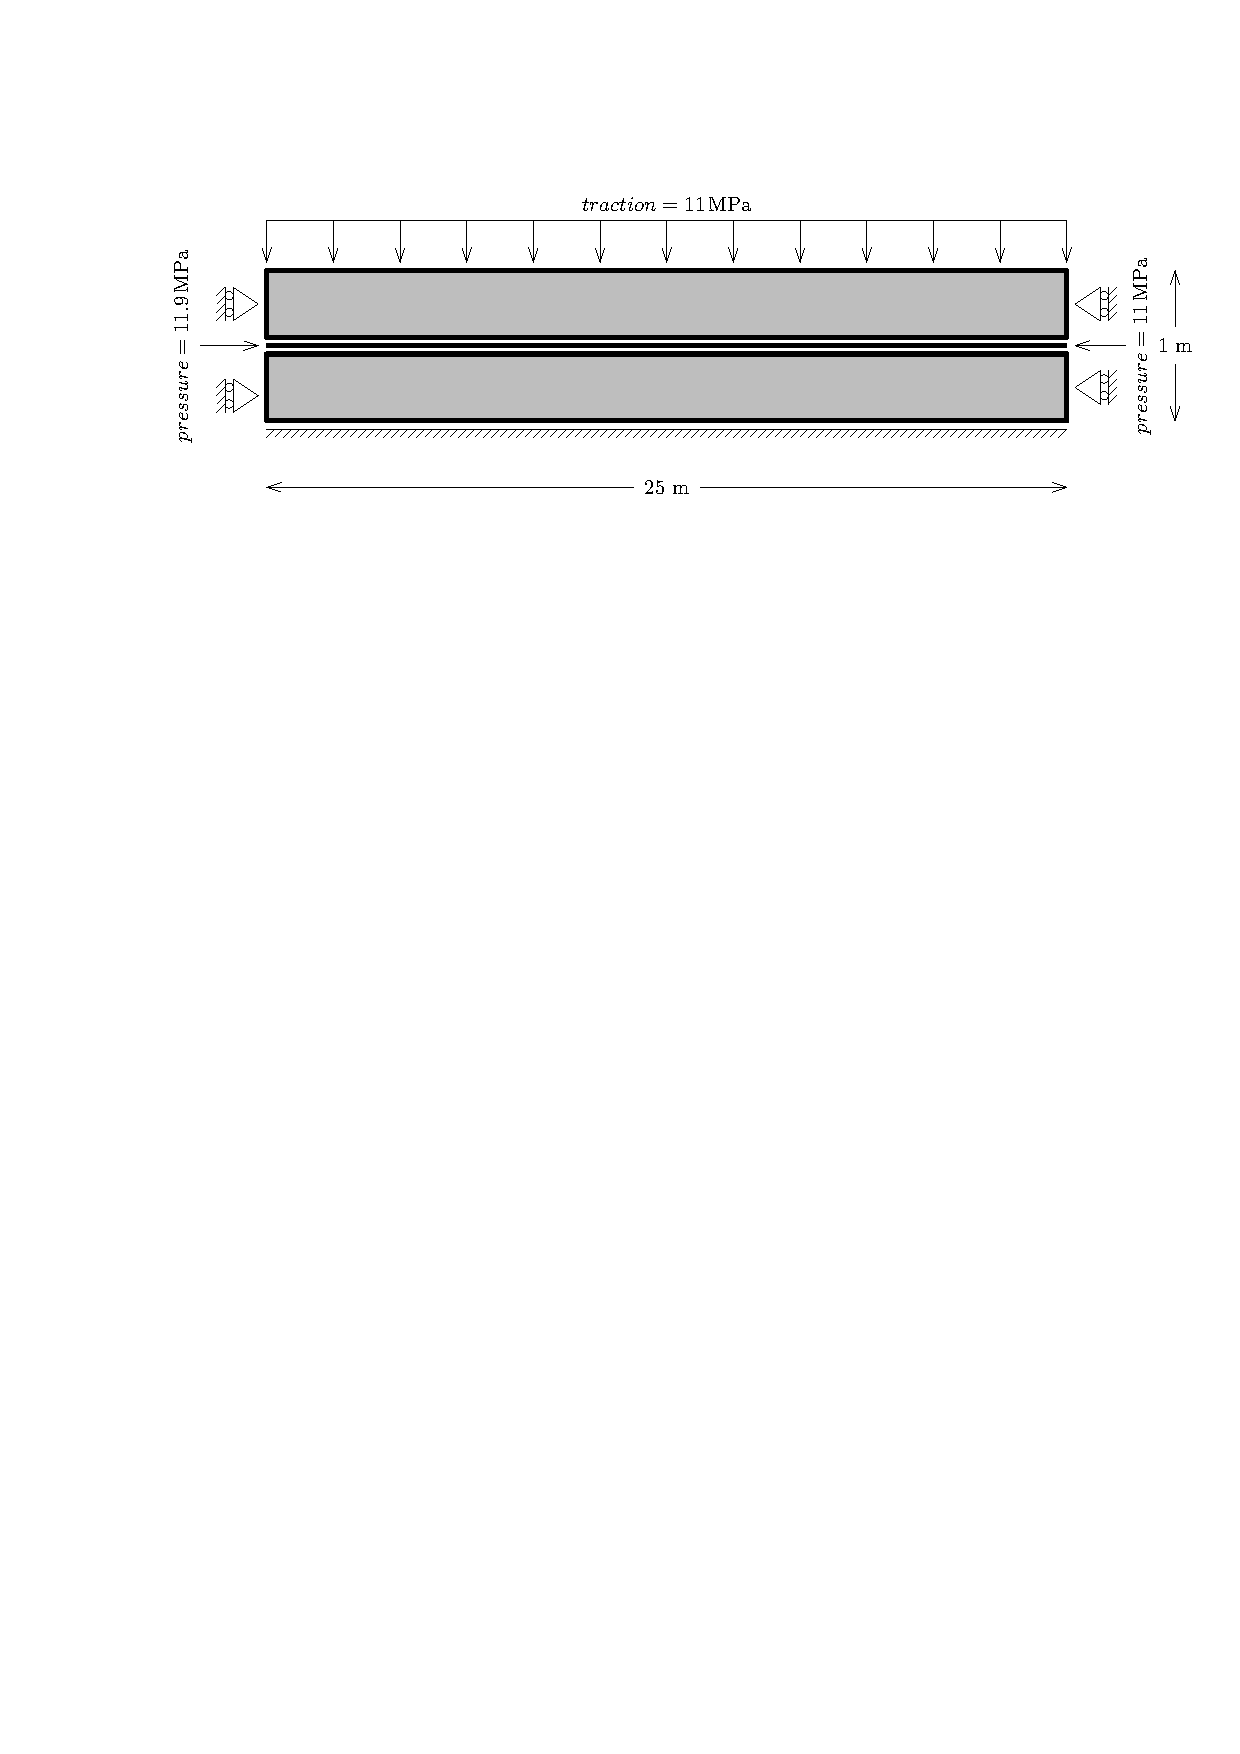
\includegraphics[width=\textwidth]{figures/test-cubic-law-bc}
\caption{Geometry and boundary conditions for the test problem.}
\label{fig:test_geom}
\end{figure}

\begin{table}
\centering
\begin{tabular}{|l|c|c|}
\hline
\bf Parameter & \multicolumn{2}{|c|}{\bf Value}\\\cline{2-3}
& \bf Matrix & \bf Fracture\\
\hline
$k$ $[\rm m^2]$ & $10^{-21}$ & $8.3\times 10^{-12}$\\
$\mu$ $[\rm Pa\, s]$ & $10^{-3}$ & $10^{-3}$\\
$S$ $[\rm Pa^{-1}]$ & $10^{-12}$ & $10^{-10}$\\
$E$ $[\rm Pa]$ & $60\times 10^9$ & $10^{6}$ \\
$\nu$ $[-]$ & 0 & 0\\
$\alpha$ $[-]$ & 1 & 1\\
$\delta$ $[\rm m]$ & --- & $10^{-5}$\\
\hline
\end{tabular}
\caption{Parameters for the test problem.}
\label{tab:test_params}
\end{table}

\subsection{Numerical solution}
The numerical scheme of the discrete fracture-matrix model has been implemented as part of the 
Flow123d simulator \cite{flow123d}, which uses conforming simplicial mixed-meshes.
The flow part of the problem is discretized using the implicit Euler timestepping and the lumped mixed hybrid finite element method \cite{Younes2006}.
%The flux, pressure and pressure trace on the sides of the elements are approximated using the $RT_0/P_0/P_0^{sides}$ finite elements.
The mechanical part is discretized using linear finite elements for the displacement.
In each discrete time, the coupled hydro-mechanical problem is solved iteratively using the fixed-stress splitting.
The iterations are stopped when the relative difference of two successive iterates drops below the given tolerance:
\eq{ \norm{P^{n}-P^{n-1}}_\Hf \le tol\norm{P^{n-1}}_\Hf. }
We refer to \cite{flow123d} for further details of the implementation.

\subsection{Results and discussion}
For the test problem, the computational mesh consists of 6856 triangular elements, and the fracture is divided into 500 lines, which coincide with sides of adjacent triangular elements.
The computational time interval is $[0,2000\,\mbox{s}]$ with the time step $\Delta t=100\,\mbox{s}$.
% 
The computed pressure profile in the fracture at selected times is depicted and compared to the analytical solution in Figure \ref{fig:test_solution}.
The results are in a good agreement.
\begin{figure}[h]
\centering
\includegraphics[width=\textwidth,ext=.png]{figures/{conv_result_linear.yaml_dt_100_cond_9.81e-18_Er_6e+10_Ef_1e+06_nur_0_nuf_0_beta_1_pressure}.pdf}
\caption{Comparison of fracture pressure given by the mixed-dimensional model and by the analytical solution.}
\label{fig:test_solution}
\end{figure}

Next, we test the iterative coupling of flow and mechanics.
Motivated by Theorem \ref{th:conv_iter}, we set
\eq{ \beta_*:=\tilde\beta\frac{\alpha_*^2}{2(\mu_*+\lambda_*)}, ~*\in\{m,f\}, }
where $\tilde\beta\in[0.3,10]$ is a scaling parameter, and study its influence on the convergence of the coupling.
The tolerance for the iterations is set to $tol=10^{-6}$.
In Figure \ref{fig:test_iterations_table} we show the dependence of number of iterations, necessary to achieve the convergence criterion, on $\tilde\beta$.
The number of iterations was averaged over all time steps and depicted together with the range between the minimal and maximal values.
\begin{figure}
\centering
\begin{subfigure}[b]{0.49\textwidth}
\centering
\includegraphics[width=\textwidth]{figures/{conv_result_linear.yaml_dt_100_alpha_1_cond_9.81e-18_Er_6e+10_Ef_1e+06_nur_0_nuf_0}.pdf}
\caption{Parameters from Table \ref{tab:test_params}.}
\label{fig:test_iterations_table}
\end{subfigure}
% \hfill
\begin{subfigure}[b]{0.49\textwidth}
\centering
\includegraphics[width=\textwidth]{figures/{conv_result_linear.yaml_dt_100_alpha_1_cond_9.81e-11_Er_6e+10_Ef_1e+06_nur_0_nuf_0}.pdf}
\caption{$k_m=10^{-14}$}
\end{subfigure}
% 
\begin{subfigure}[b]{0.49\textwidth}
\centering
\includegraphics[width=\textwidth]{figures/{conv_result_linear.yaml_dt_100_alpha_1_cond_9.81e-05_Er_6e+10_Ef_1e+06_nur_0_nuf_0}.pdf}
\caption{$k_m=10^{-8}$}
\end{subfigure}
% 
\begin{subfigure}[b]{0.49\textwidth}
\centering
\includegraphics[width=\textwidth]{figures/{conv_result_linear.yaml_dt_100_alpha_1_cond_9.81e-18_Er_6e+10_Ef_1e+06_nur_0.25_nuf_0.25}.pdf}
\caption{$\nu_m=\nu_f=0.25$}
\end{subfigure}
% 
\begin{subfigure}[b]{0.49\textwidth}
\centering
\includegraphics[width=\textwidth]{figures/{conv_result_linear.yaml_dt_100_alpha_1_cond_9.81e-18_Er_6e+10_Ef_1e+06_nur_0.49_nuf_0.49}.pdf}
\caption{$\nu_m=\nu_f=0.49$}
\end{subfigure}
% 
\begin{subfigure}[b]{0.49\textwidth}
\centering
\includegraphics[width=\textwidth]{figures/{conv_result_linear.yaml_dt_100_alpha_1_cond_9.81e-18_Er_6e+10_Ef_1e+09_nur_0_nuf_0}.pdf}
\caption{$E_f=10^{9}$}
\end{subfigure}
\caption{Convergence of iterative splitting. Number of iterations necessary for meeting the stopping criterion is depicted for several parameter cases. The filled area indicates the range of iteration counts for all time steps, the line shows the average number of iterations.}
\label{fig:test_iterations}
\end{figure}
It turns out that, in agreement with Theorem \ref{th:conv_iter}, the optimal value of $\tilde\beta$ is close to 1.
Moreover, its overestimation leads to moderate increase of number of iterations while for $\tilde\beta<1$ the iterative scheme converges very slowly or diverges.
To verify the robustness of the estimate \eqref{eq:cond_beta}, we performed analogous tests for perturbed conductivity, and elastic moduli, see Figure \ref{fig:test_iterations}.
From the results it can be seen that the optimal choice of $\tilde\beta$ is in all cases either 1 or slightly larger, which confirms the theoretical estimates.


\section*{Conclusion}
We have derived a mixed-dimensional model of flow and linear elasticity in fractured porous media.
The model was derived from physical principles expressed by the Biot system and takes into account possible anisotropy of the hydraulic conductivity and elasticity tensors.
A simplified geometry consisting of one straight fracture was considered.

Under the assumption of permeable fracture, the existence and uniqueness of weak solution was proved.
The proof was based on the fixed-stress splitting scheme for which the convergence has been analyzed and optimal values of iteration parameters were found in as similar form as in \cite{both2017robust}.

A numerical test was presented that confirmed the theoretical convergence result of the splitting scheme as well as the applicability of the mixed-dimensional model.
The analysis of the numerical scheme is beyond the scope of the present paper.

The model can be extended in many directions, namely to more complex geometries (embedded fractures with variable aperture and their intersections), nonlinear fracture mechanics \cite{berge2019finite}, or variable fracture permeability \cite{Watanabe2012lower}, to name a few challenging tasks.
Some of these have been implemented in the Flow123d simulator, others are a subject of ongoing research.


\section*{Acknowledgement}
The research was supported by the Euratom research and training programme 2014-2018 under grant agreement No [847593].

\appendix
\titlelabel{Appendix \thetitle.\hspace{0.5em}}
% \section{Appendix}

\section{Auxiliary inequalities and identities}\label{sec:ap_ineq}

In what follows we prove some technical relations that are used in the paper.
\begin{lemma}\label{th:eq_avg_grads}
For all admissible functions $f$, $\vv$ and $\tn A$ it holds:
\begin{align*}
\overline{\nabla f} &= \nabla_\tau\overline f + \frac1\delta\jmp{f}\nnu = \avg{\agrad(f,\overline f)}, \\
\overline{\nabla\vv} &= \nabla_\tau\overline\vv+\frac1\delta\jmp{\vv}\otimes\nnu = \avg{\agrad(\vv,\overline\vv)}, \\
\overline{\div\vv} &= \div_\tau\overline\vv+\frac1\delta\jmp{\vv}\cdot\nnu = \avg{\adiv(\vv,\overline\vv)}, \\
\overline{\div\tn A} &= \div_\tau\overline{\tn A} + \frac1\delta\jmp{\tn A^\top}\nnu.
\end{align*}
\end{lemma}
\begin{proof}
It is readily seen that $\avg{\agrad(f,\overline f)}=\nabla_\tau\overline f + \frac1\delta\jmp{f}$.
Further we have:
\eqs{ \overline{\nabla_\tau f} = \frac1\delta\int_{-\tfrac\delta2}^{\tfrac\delta2}\nabla_\tau f(\cdot+s\nnu) \d s = \nabla_\tau\left(\frac1\delta\int_{-\tfrac\delta2}^{\tfrac\delta2}f(\cdot+s\nnu) \d s\right) = \nabla_\tau\overline f,
}
\eqs{ \overline{\nabla_\nu f} = \frac1\delta\int_{-\tfrac\delta2}^{\tfrac\delta2}\nnu\frac{\rm d}{{\rm d}s}\left(f(\cdot+s\nnu)\right)\d s = \frac1\delta\jmp{f}\nnu,
}
so that $\overline{\nabla f} = \overline{\nabla_\tau f} + \overline{\nabla_\nu f} = \avg{\agrad(f,\overline f)}$.
The remaining identities can be proved analogously.
\end{proof}


\begin{lemma}
For all functions $\V:=(\V_m,\V_f)\in\Vel$ it holds:
\eq{ \label{eq:ineq_div_ep} \norm{\div\V_m}_{L^2(\Omega_m)}^2 \le d\norm{\ep(\V_m)}_{L^2(\Omega_m)}^2, }
\eq{ \label{eq:ineq_adiv_aep} \norm{\adiv^\opm\V}_{L^2(\gamma)}^2 \le d\norm{\aep^\opm(\V)}_{L^2(\gamma)}^2. }
\end{lemma}
\begin{proof}
For any tensor $\tn A\in\Real^{d\times d}$, the AM-QM inequality implies
\eqs{ |\tn I:\tn A|^2 \le d|\tn A|^2. }
Choosing $\tn A:=\ep(\V_m)$ and integrating the inequality over $\Omega_m$ we obtain \eqref{eq:ineq_div_ep}.
Similarly, \eqref{eq:ineq_adiv_aep} is obtained for $\tn A:=\aep^\opm(\V)$ and integration over $\gamma$.
\end{proof}


\begin{lemma}
The functions $\ttraction^\opm$ and $\varphi^\opm$, defined in \eqref{eq:def_t} and \eqref{eq:def_F}, satisfy:
\eq{ \label{eq:ellip_t} \jmp{\ttraction(\V)\cdot(\vc W_m-\vc W_f)} = \delta\avg{\CC_f\agrad\V:\agrad_\nu{\vc W}}, }
\eq{ \label{eq:ellip_phi} \jmp{\varphi(Q)(R_m-R_f)} = \delta\avg{\tn K_f\agrad Q\cdot\agrad_\nu R} }
for all admissible functions $\V:=(\V_m,\V_f)$, $\vc W:=(\vc W_m,\vc W_f)$, $Q:=(Q_m,Q_f)$ and $R:=(R_m,R_f)$.
\end{lemma}
\begin{proof}
From the definition of $\ttraction^\opm$ and $\agrad^\opm$ it follows that
\mls{ \ttraction^\opm(\V)\cdot(\vc W_m^\opm-\vc W_f)
= \pm\frac\delta2\CC_f\agrad^\opm\V:\left(\pm\frac2\delta\right)(\vc W_m^\opm-\vc W_f)\otimes\nnu\\
= \pm\frac\delta2\CC_f\agrad^\opm\V:\agrad_\nu^\opm\vc W. }
Taking the jump of the above expression then yields \eqref{eq:ellip_t}.
The second identity can be proved in analogous way.
\end{proof}


% \section{Energy equality for \eqref{eq:mixed_dim_problem}}\label{sec:app_energy_eq}
% 
% In this section we derive the identity \eqref{eq:apriori_biot}.
% Assuming that $(\U,P)$ is a smooth solution of \eqref{eq:mixed_dim_problem}, we take the time derivative of \eqref{eq:mixed_dim_problem_el_mat}, multiply by $\dt{\U_m}$ and integrate over $\Omega_m$.
% Then we apply the Green identity, interface and boundary conditions \eqref{eq:mixed_dim_problem_int_el}, \eqref{eq:mixed_dim_problem_bc}, which yields:
% \ml{ \label{eq:energy_el_mat} \int_{\Omega_m}(\CC_m\nabla\dt{\U_m}:\nabla\dt{\U_m} - \alpha_m\dt P_m \div\dt{\U_m}) + \int_\gamma\jmp{\ttraction(\dt\U)\cdot\dt{\U_m}}\\
% - \int_\gamma\alpha_f\dt P_f\jmp{\dt{\U_m}}\cdot\nnu
% = \dual{\dt\FF_m}{\dt{\U_m}}_{H^1_\Gamma(\Omega_m;\Real^d)}. }
% Similarly we differentiate \eqref{eq:mixed_dim_problem_el_frac} with respect to time, multiply by $\dt{\U_f}$, integrate over $\gamma$, use Green's formula and apply the boundary conditions \eqref{eq:mixed_dim_problem_bc}.
% We arrive at the identity
% \ml{ \label{eq:energy_el_frac} \delta\int_\gamma\CC_f\avg{\agrad\dt\U}:\nabla_\tau\dt{\U_f} - \delta\int_\gamma\alpha_f\dt P_f\div_\tau\dt{\U_f}\\
% % + \int_\gamma\alpha_f\jmp{\dt P_m}\dt{\U_f}\cdot\nnu
% - \int_\gamma\jmp{\ttraction(\dt\U)}\cdot\dt{\U_f} = \dual{\dt\FF_f}{\dt{\U_f}}_{H^1_0(\gamma;\Real^d)}. }
% Next we multiply \eqref{eq:mixed_dim_problem_fl_mat} by $\dt P_m$ and \eqref{eq:mixed_dim_problem_fl_frac} by $\dt P_f$, integrate over $\Omega_m$, $\gamma$, respectively, use Green's formula, interface and boundary conditions \eqref{eq:mixed_dim_problem_int_fl}, \eqref{eq:mixed_dim_problem_bc}.
% We get the following equalities:
% \ml{ \label{eq:energy_fl_mat} S_m\int_{\Omega_m}|\dt P_m|^2 + \int_{\Omega_m}\alpha_m\dt P_m\div\dt{\U_m} + \int_\gamma\jmp{\varphi(P)\dt P_m}\\
% + \frac12\ddt{}\int_{\Omega_m}\tn K_m\nabla P_m\cdot\nabla P_m
% = \dual{G_m}{\dt P_m}_{H^1_\Gamma(\Omega_m)}, }
% \ml{ \label{eq:energy_fl_frac} \delta S_f\int_\gamma|\dt P_f|^2 + \delta\int_\gamma\alpha_f\dt P_f\div_\tau\dt{\U_f} + \int_\gamma\alpha_f\dt P_f\jmp{\dt{\U_m}}\cdot\nnu\\
% + \delta\int_\gamma\tn K_f\avg{\agrad P}\cdot\nabla_\tau\dt P_f 
% - \int_\gamma\jmp{\varphi(P)}\dt P_f = \dual{G_f}{\dt P_f}_{H^1_0(\gamma)}. }
% Summing up \eqref{eq:energy_el_mat}--\eqref{eq:energy_fl_frac} some terms cancel out and we obtain:
% \ml{ \label{eq:energy_sum} \int_{\Omega_m}(\CC_m\nabla\dt{\U_m}:\nabla\dt{\U_m} ) + \int_\gamma\jmp{\ttraction(\dt\U)\cdot\dt({\U_m}-{\U_f})}\\
% % - \int_\gamma\alpha_f\jmp{\dt P_m \dt{\U_m}}\cdot\nnu
% + \delta\int_\gamma\CC_f\avg{\agrad\dt\U}:\nabla_\tau\dt{\U_f}
% % + \int_\gamma\alpha_f\jmp{\dt P_m}\dt{\U_f}\cdot\nnu
% + S_m\int_{\Omega_m}|\dt P_m|^2\\
% + \int_\gamma\jmp{\varphi(P)\dt(P_m-P_f)}
% + \frac12\ddt{}\int_{\Omega_m}\tn K_m\nabla P_m\cdot\nabla P_m
% + \delta S_f\int_\gamma|\dt P_f|^2
% % + \int_\gamma\alpha_f\dt P_f\jmp{\dt{\U_m}}\cdot\nnu
% \\
% + \delta\int_\gamma\tn K_f\avg{\agrad P}\cdot\nabla_\tau\dt P_f 
% = \dual{\dt\FF}{\dt{\U_m}}_{\Vel} + \dual{G}{\dt P_m}_{\Vf}. }
% Using \eqref{eq:ellip_t}--\eqref{eq:ellip_phi} in \eqref{eq:energy_sum} leads to the identity
% \mls{ \int_{\Omega_m}(\CC_m\nabla\dt{\U_m}:\nabla\dt{\U_m} ) + \delta\int_\gamma\avg{\CC_f\agrad\dt\U:\agrad\dt\U}\\
% + S_m\int_{\Omega_m}|\dt P_m|^2 + \delta S_f\int_\gamma|\dt P_f|^2\\
% + \frac12\ddt{}\int_{\Omega_m}\tn K_m\nabla P_m\cdot\nabla P_m
% + \delta\int_\gamma\avg{\tn K_f\agrad P\cdot\agrad\dt P} \\
% % - \int_\gamma\alpha_f\jmp{\dt P_m \dt{\U_m}}\cdot\nnu
% % + \int_\gamma\alpha_f\jmp{\dt P_m}\dt{\U_f}\cdot\nnu
% % + \int_\gamma\alpha_f\dt P_f\jmp{\dt{\U_m}}\cdot\nnu\\
% = \dual{\dt\FF}{\dt{\U_m}}_{\Vel} + \dual{G}{\dt P_m}_{\Vf}, }
% which is in fact \eqref{eq:apriori_biot}.



\section{Weak formulation of \eqref{eq:mixed_dim_problem}}\label{sec:app_weak_form}

In what follows we derive the integral identities (\ref{eq:biot_weak-ii}) -- (\ref{eq:biot_weak-iii}).
Multiplying \eqref{eq:mixed_dim_problem_el_mat} and \eqref{eq:mixed_dim_problem_el_frac} by test functions $\V_m$, $\V_f$, respectively, where $\V:=(\V_m,\V_f)\in\Vel$, integrating them by parts, summing and applying the boundary conditions \eqref{eq:mixed_dim_problem_bc}, we arrive at the identity
\ml{ \label{eq:mixed_el_integrated} \int_{\Omega_m}\left(\CC_m\nabla{\U_m}:\nabla\V_m - \alpha_m P_m\div\V_m\right)
 + \int_\gamma\jmp{(\CC_m\nabla{\U_m}-\alpha_m P_m\tn I)\nnu\cdot\V_m}\\
 + \delta\int_\gamma\CC_f\avg{\agrad\U}:\nabla_\tau\V_f
 - \int_\gamma \alpha_f\delta P_f \div_\tau\V_f
 - \int_\gamma \jmp{\ttraction(\U)\cdot\V_f}\\
 = \dual{\FF}{\V}_\Vel. }
 The second term in \eqref{eq:mixed_el_integrated} can be rewritten using the interface conditions \eqref{eq:mixed_dim_problem_int_el}, which yields:
\ml{ \label{eq:mixed_el_integrated_int} \int_{\Omega_m}\left(\CC_m\nabla{\U_m}:\nabla\V_m - \alpha_m P_m\div\V_m\right)
 + \delta\int_\gamma\CC_f\avg{\agrad\U}:\nabla_\tau\V_f\\
 + \int_\gamma \jmp{\ttraction(\U)\cdot(\V_m-\V_f)}
 - \delta\int_\gamma \alpha_f P_f\avg{\adiv\V}
 = \dual{\FF}{\V}_\Vel. }
Using \eqref{eq:ellip_t}, we can rewrite \eqref{eq:mixed_el_integrated_int} as follows:
\mls{ \int_{\Omega_m}\left(\CC_m\nabla{\U_m}:\nabla\V_m - \alpha_m P_m\div\V_m\right)\\
 + \delta\int_\gamma\avg{\CC_f\agrad\U:\agrad\V-\alpha_f P_f \adiv\V}
  = \dual{\FF}{\V}_\Vel, }
which is \eqref{eq:biot_weak-ii}.
Similarly, multiplying the equations \eqref{eq:mixed_dim_problem_fl_mat}, \eqref{eq:mixed_dim_problem_fl_frac} by test functions $Q_m$, $Q_f$, respectively, where $Q:=(Q_m,Q_f)\in\Vf$, integrating them by parts, and applying the boundary conditions \eqref{eq:mixed_dim_problem_bc}, we obtain:
\mls{ \int_{\Omega_m}\left(Q_m\dt(S_m P_m+\alpha_m\div{\U_m}) + \tn K_m\nabla P_m\cdot\nabla Q_m\right) + \int_\gamma\jmp{\tn K_m\nabla P_m\cdot\nnu Q_m}\\
+ \delta \int_\gamma Q_f\dt\left(S_f P_f + \alpha_f\avg{\adiv\U}\right)
+ \delta \int_\gamma \tn K_f\avg{\agrad P}\cdot\nabla_\tau Q_f\\
- \int_\gamma \jmp{\pphi(P)}Q_f
= \dual{G}{Q}_\Hf. }
Application of the interface conditions \eqref{eq:mixed_dim_problem_int_fl} then gives rise to the identity
\ml{ \label{eq:mixed_fl_integrated_int} \int_{\Omega_m}\left(Q_m\dt(S_m P_m+\alpha_m\div{\U_m}) + \tn K_m\nabla P_m\cdot\nabla Q_m\right)\\
+ \delta \int_\gamma Q_f\dt\left(S_f P_f + \alpha_f\avg{\adiv\U}\right)
+ \delta \int_\gamma \tn K_f\avg{\agrad P}\cdot\nabla_\tau Q_f\\
+ \int_\gamma \jmp{\pphi(P)(Q_m-Q_f)}
= \dual{G}{Q}_\Hf. }
Due to \eqref{eq:ellip_phi}, \eqref{eq:mixed_fl_integrated_int} becomes
\mls{ \int_{\Omega_m}\left(Q_m\dt(S_m P_m+\alpha_m\div{\U_m}) + \tn K_m\nabla P_m\cdot\nabla Q_m\right)\\
+ \delta \int_\gamma Q_f\dt\left(S_f P_f + \alpha_f\avg{\adiv\U}\right)
+ \delta \int_\gamma \avg{\tn K_f\agrad P\cdot\agrad Q}
= \dual{G}{Q}_\Hf, }
which is \eqref{eq:biot_weak-iii}.

The energy equality \eqref{eq:apriori_biot} can be obtained from the weak formulation as follows.
One has to differentiate \eqref{eq:biot_weak-ii} with respect to time, test by $\V:=\dt\U$ and add to \eqref{eq:biot_weak-iii} tested by $Q:=\dt P$.






\bibliographystyle{abbrvnat}
\bibliography{biot_fracture.bib}

\end{document}


